\documentclass[11pt, oneside]{article}   	% use "amsart" instead of "article" for AMSLaTeX format
\usepackage{geometry}                		% See geometry.pdf to learn the layout options. There are lots.
\geometry{letterpaper}                   		% ... or a4paper or a5paper or ... 
%\geometry{landscape}                		% Activate for rotated page geometry
\usepackage[parfill]{parskip}    		% Activate to begin paragraphs with an empty line rather than an indent
\usepackage{graphicx}				% Use pdf, png, jpg, or eps§ with pdflatex; use eps in DVI mode
								% TeX will automatically convert eps --> pdf in pdflatex		
\usepackage[margin=10pt,font=footnotesize,labelfont=bf]{caption}
\usepackage{subcaption}
\usepackage{float}
\usepackage{amssymb}
\usepackage{amsmath}
\usepackage{bm}
\usepackage{bbm}
\usepackage{mleftright}
\usepackage{todonotes}

%\bibliographystyle{apalike}

\graphicspath{ {images/} }

\newcommand{\sotodo}{\todo[color=green]}
\newcommand{\sotodoinline}{\todo[color=green,inline=true]}
\newcommand{\bstodo}{\todo[color=pink]}
\newcommand{\bstodoinline}{\todo[color=pink,inline=true]}


%SetFonts

%SetFonts

\usepackage[square,numbers]{natbib}
\usepackage{url}
%\bibliographystyle{elsarticle-harv}
\bibliographystyle{plain}

\newcommand{\bigO}{\mathcal{O}}
\newcommand{\half}{\frac{1}{2}}
\newcommand{\R}{\mathbb{R}}
\newcommand{\C}{\mathbb{C}}
\newcommand{\Z}{\mathbb{Z}}
\newcommand{\N}{\mathbb{N}}
\newcommand{\No}{\mathbb{N}_0}
\newcommand{\Ylm}{Y^m_l}
\newcommand{\Ylmfull}{Y^m_l(\theta,\varphi)}
\newcommand{\Plm}{\jac^m_l}
\newcommand{\costheta}{\cos\theta}
\newcommand{\sintheta}{\sin\theta}
\newcommand{\cosphi}{\cos\varphi}
\newcommand{\sinphi}{\sin\varphi}
\newcommand{\eimphi}{e^{im\varphi}}
\newcommand{\alphalm}{\alpha^m_l}
\newcommand{\clm}{c^m_l}
\newcommand{\ctilde}{\tilde{c}^m_l}
\newcommand{\ctildemod}{\tilde{c}^{|m|}_l}
\newcommand{\chat}{\hat{c}^m_l}
\newcommand{\chatmod}{\hat{c}^{|m|}_l}
\newcommand{\ddx}{\frac{\mathrm{d}}{\mathrm{d}x}}
\newcommand{\ddy}{\frac{\mathrm{d}}{\mathrm{d}y}}
\newcommand{\pddx}{\frac{\partial}{\partial x}}
\newcommand{\pddy}{\frac{\partial}{\partial y}}
\newcommand{\pddn}{\frac{\partial}{\partial n}}
\newcommand{\dmdxm}{\frac{\mathrm{d}^m}{\mathrm{d}x^m}}

\newcommand{\Atilde}{\tilde{A}_{l,m}}
\newcommand{\Btilde}{\tilde{B}_{l,m}}
\newcommand{\Dtilde}{\tilde{D}_{l,m}}
\newcommand{\Etilde}{\tilde{E}_{l,m}}
\newcommand{\Ftilde}{\tilde{F}_{l,m}}
\newcommand{\Gtilde}{\tilde{G}_{l,m}}
\newcommand{\Alm}{A_{l,m}}
\newcommand{\Blm}{B_{l,m}}
\newcommand{\Dlm}{D_{l,m}}
\newcommand{\Elm}{E_{l,m}}
\newcommand{\Flm}{F_{l,m}}
\newcommand{\Glm}{G_{l,m}}

\newcommand{\xione}{\xi^{(1)}_{n, \lambda}}
\newcommand{\xitwo}{\xi^{(2)}_{n, \lambda}}
\newcommand{\xithree}{\xi^{(3)}_{n, \lambda}}
\newcommand{\xifour}{\xi^{(4)}_{n, \lambda}}

\newcommand{\bigP}{\mathbb{P}}
\newcommand{\Pl}{\mathbb{P}_l}
\newcommand{\gradP}{T\mathbb{P}}
\newcommand{\gradPl}{T\mathbb{P}_l}
\newcommand{\gradY}{\nabla Y}
\newcommand{\gradYlm}{\nabla Y^m_l}
\newcommand{\gradpY}{\nabla^\perp Y}
\newcommand{\gradpYlm}{\nabla^\perp Y^m_l}

\newcommand{\Dlt}{D^\top_l}

\newcommand{\curlyy}{\bm{\mathcal{Y}}}
\newcommand{\blone}{\beta_{l, 1}}
\newcommand{\blzero}{\beta_{l, 0}}
\newcommand{\blmone}{\beta_{l, -1}}
\newcommand{\chivec}{\bm{\chi}_{1,m_s}}
\newcommand{\cgcoeff}{\mathcal{C}}

\newcommand{\alm}{a_{l,m}}
\newcommand{\blm}{b_{l,m}}
\newcommand{\dlm}{d_{l,m}}
\newcommand{\elm}{e_{l,m}}
\newcommand{\flm}{f_{l,m}}
\newcommand{\glm}{g_{l,m}}
\newcommand{\hlm}{h_{l,m}}
\newcommand{\jlm}{j_{l,m}}
\newcommand{\klm}{k_{l,m}}
\newcommand{\almperp}{a_{l,m}^\perp}
\newcommand{\blmperp}{b_{l,m}^\perp}
\newcommand{\dlmperp}{d_{l,m}^\perp}
\newcommand{\elmperp}{e_{l,m}^\perp}
\newcommand{\flmperp}{f_{l,m}^\perp}
\newcommand{\glmperp}{g_{l,m}^\perp}
\newcommand{\hlmperp}{h_{l,m}^\perp}
\newcommand{\jlmperp}{j_{l,m}^\perp}
\newcommand{\klmperp}{k_{l,m}^\perp}

\newcommand{\unitvec}{\hat{\bm{k}}}

\newcommand{\hdop}{H}
\newcommand{\bighdop}{\mathbb{\hdop}}
\newcommand{\hdopnk}{\hdop_{n,k}}
\newcommand{\hdopab}{\hdop^{(a,b)}}
\newcommand{\hdopnkab}{\hdop_{n,k}^{(a,b)}}
\newcommand{\Wab}{{W^{(a,b)}}}
\newcommand{\hdopmj}{\hdop_{m,j}}
\newcommand{\hdopmjab}{\hdop_{m,j}^{(a,b)}}
\newcommand{\alphaab}{\alpha^{(a,b)}}
\newcommand{\betaab}{\beta^{(a,b)}}
\newcommand{\bighdopab}{\bighdop^{(a,b)}}
\newcommand{\Dnt}{D^\top_n}
\newcommand{\Wii}{W^{(1,1)}}
\newcommand{\hdopii}{\hdop^{(1,1)}}
\newcommand{\bighdopii}{{\mathbb{\hdop}^{(1,1)}}}
\newcommand{\hdopoo}{\hdop^{(0,0)}}
\newcommand{\bighdopoo}{{\mathbb{\hdop}^{(0,0)}}}
\newcommand{\hdopoi}{\hdop^{(0,1)}}
\newcommand{\hdopio}{\hdop^{(1,0)}}
\newcommand{\jac}{{\tilde P}}
\newcommand{\genjac}{R}
\newcommand{\genjacnmk}{\genjac_{n-k}}
\newcommand{\genjacmmj}{\genjac_{m-j}}
\newcommand{\genjacw}{w_\genjac}
\newcommand{\jacw}{w_P}
\newcommand{\normgenjac}{\omega_\genjac}
\newcommand{\normjac}{\omega_P}


\newcommand{\dx}{\frac{\partial}{\partial x}}
\newcommand{\dy}{\frac{\partial}{\partial y}}
\newcommand{\laplacewii}{\Delta_W^{(1,1)\to(1,1)}}
\newcommand{\laplacewtt}{\Delta_W^{(2,2)\to(0,0)}}
\newcommand{\laplaceoo}{\Delta^{(0,0)\to(2,2)}}
\newcommand{\biharmonic}{_2\Delta_W^{(2,2)\to(2,2)}}

\newcommand{\element}{\tau}
\newcommand{\refelement}{\hat{\tau}}
\newcommand{\FEset}{\mathcal{T}}
\newcommand{\bigW}{\mathbb{W}}
\newcommand{\bigWab}{\mathbb{W}^{(a,b)}}
\newcommand{\bigWii}{{\mathbb{W}^{(1,1)}}}
\newcommand{\bigQ}{\mathbb{Q}}
\newcommand{\bigQab}{\bigQ^{(a,b)}}

\usepackage{amsthm}

\newtheorem{proposition}{Proposition}
\newtheorem{lemma}{Lemma} 
\newtheorem{theorem}{Theorem} 
\newtheorem{definition}{Definition}
\newtheorem{algorithm}{Algorithm}


\def\addtab#1={#1\;&=}

\def\meeq#1{\def\ccr{\\\addtab}
%\tabskip=\@centering
 \begin{align*}
 \addtab#1
 \end{align*}
  }  
  
  \def\leqaddtab#1\leq{#1\;&\leq}
  \def\mleeq#1{\def\ccr{\\\addtab}
%\tabskip=\@centering
 \begin{align*}
 \leqaddtab#1
 \end{align*}
  }  


\def\vc#1{\mbox{\boldmath$#1$\unboldmath}}

\def\vcsmall#1{\mbox{\boldmath$\scriptstyle #1$\unboldmath}}

\def\vczero{{\mathbf 0}}


%\def\beginlist{\begin{itemize}}
%
%\def\endlist{\end{itemize}}


\def\pr(#1){\left({#1}\right)}
\def\br[#1]{\left[{#1}\right]}
\def\fbr[#1]{\!\left[{#1}\right]}
\def\set#1{\left\{{#1}\right\}}
\def\ip<#1>{\left\langle{#1}\right\rangle}
\def\iip<#1>{\left\langle\!\langle{#1}\right\rangle\!\rangle}

\def\norm#1{\left\| #1 \right\|}

\def\abs#1{\left|{#1}\right|}
\def\fpr(#1){\!\pr({#1})}

\def\Re{{\rm Re}\,}
\def\Im{{\rm Im}\,}

\def\floor#1{\left\lfloor#1\right\rfloor}
\def\ceil#1{\left\lceil#1\right\rceil}


\def\mapengine#1,#2.{\mapfunction{#1}\ifx\void#2\else\mapengine #2.\fi }

\def\map[#1]{\mapengine #1,\void.}

\def\mapenginesep_#1#2,#3.{\mapfunction{#2}\ifx\void#3\else#1\mapengine #3.\fi }

\def\mapsep_#1[#2]{\mapenginesep_{#1}#2,\void.}


\def\vcbr[#1]{\pr(#1)}


\def\bvect[#1,#2]{
{
\def\dots{\cdots}
\def\mapfunction##1{\ | \  ##1}
	\sopmatrix{
		 \,#1\map[#2]\,
	}
}
}

\def\vect[#1]{
{\def\dots{\ldots}
	\vcbr[{#1}]
}}

\def\vectt[#1]{
{\def\dots{\ldots}
	\vect[{#1}]^{\top}
}}

\def\Vectt[#1]{
{
\def\mapfunction##1{##1 \cr} 
\def\dots{\vdots}
	\begin{pmatrix}
		\map[#1]
	\end{pmatrix}
}}



\def\thetaB{\mbox{\boldmath$\theta$}}
\def\zetaB{\mbox{\boldmath$\zeta$}}


\def\newterm#1{{\it #1}\index{#1}}


\def\TT{{\mathbb T}}
\def\C{{\mathbb C}}
\def\R{{\mathbb R}}
\def\II{{\mathbb I}}
\def\F{{\mathcal F}}
\def\E{{\rm e}}
\def\I{{\rm i}}
\def\D{{\rm d}}
\def\dx{\D x}
\def\dy{\D y}
\def\CC{{\cal C}}
\def\DD{{\cal D}}
\def\U{{\mathbb U}}
\def\A{{\cal A}}
\def\K{{\cal K}}
\def\DTU{{\cal D}_{{\rm T} \rightarrow {\rm U}}}
\def\LL{{\cal L}}
\def\B{{\cal B}}
\def\T{{\cal T}}
\def\W{{\cal W}}


\def\tF_#1{{\tt F}_{#1}}
\def\Fm{\tF_m}
\def\Fab{\tF_{\alpha,\beta}}
\def\FC{\T}
\def\FCpmz{\FC^{\pm {\rm z}}}
\def\FCz{\FC^{\rm z}}

\def\tFC_#1{{\tt T}_{#1}}
\def\FCn{\tFC_n}

\def\rmz{{\rm z}}

\def\chapref#1{Chapter~\ref{Chapter:#1}}
\def\secref#1{Section~\ref{Section:#1}}
\def\exref#1{Exercise~\ref{Exercise:#1}}
\def\lmref#1{Lemma~\ref{Lemma:#1}}
\def\propref#1{Proposition~\ref{Proposition:#1}}
\def\warnref#1{Warning~\ref{Warning:#1}}
\def\thref#1{Theorem~\ref{Theorem:#1}}
\def\defref#1{Definition~\ref{Definition:#1}}
\def\probref#1{Problem~\ref{Problem:#1}}
\def\corref#1{Corollary~\ref{Corollary:#1}}
\def\appref#1{Appendix~\ref{Appendix:#1}}

\def\sgn{{\rm sgn}\,}
\def\Ai{{\rm Ai}\,}
\def\Bi{{\rm Bi}\,}
\def\wind{{\rm wind}\,}
\def\erf{{\rm erf}\,}
\def\erfc{{\rm erfc}\,}
\def\qqquad{\qquad\quad}
\def\qqqquad{\qquad\qquad}


\def\spand{\hbox{ and }}
\def\spodd{\hbox{ odd}}
\def\speven{\hbox{ even}}
\def\qand{\quad\hbox{and}\quad}
\def\qqand{\qquad\hbox{and}\qquad}
\def\qfor{\quad\hbox{for}\quad}
\def\qqfor{\qquad\hbox{for}\qquad}
\def\qas{\quad\hbox{as}\quad}
\def\qqas{\qquad\hbox{as}\qquad}
\def\qor{\quad\hbox{or}\quad}
\def\qqor{\qquad\hbox{or}\qquad}
\def\qqwhere{\qquad\hbox{where}\qquad}



%%% Words

\def\naive{na\"\i ve\xspace}
\def\Jmap{Joukowsky map\xspace}
\def\Mobius{M\"obius\xspace}
\def\Holder{H\"older\xspace}
\def\Mathematica{{\sc Mathematica}\xspace}
\def\apriori{apriori\xspace}
\def\WHf{Weiner--Hopf factorization\xspace}
\def\WHfs{Weiner--Hopf factorizations\xspace}

\def\Jup{J_\uparrow^{-1}}
\def\Jdown{J_\downarrow^{-1}}
\def\Jin{J_+^{-1}}
\def\Jout{J_-^{-1}}



\def\bD{\D\!\!\!^-}




\def\questionequals{= \!\!\!\!\!\!{\scriptstyle ? \atop }\,\,\,}

\def\elll#1{\ell^{\lambda,#1}}
\def\elllp{\ell^{\lambda,p}}
\def\elllRp{\ell^{(\lambda,R),p}}


\def\elllRpz_#1{\ell_{#1{\rm z}}^{(\lambda,R),p}}


\def\sopmatrix#1{\begin{pmatrix}#1\end{pmatrix}}

\def\socases#1{\begin{cases} #1 \end{cases}}


\def\Problem#1#2\par{\begin{problem}\label{pb:#1} #2\end{problem}}
\def\Theorem#1#2\par{\begin{theorem}\label{th:#1} #2\end{theorem}}
\def\Conjecture#1#2\par{\begin{conjecture}\label{conj:#1} #2\end{conjecture}}
\def\Proposition#1#2\par{\begin{proposition}\label{prop:#1} #2\end{proposition}}
\def\Definition#1#2\par{\begin{definition}\label{def:#1} #2\end{definition}}
\def\Corollary#1#2\par{\begin{corollary}\label{cr:#1} #2\end{corollary}}
\def\Lemma#1#2\par{\begin{lemma}\label{lm:#1} #2\end{lemma}}
\def\Example#1#2\par{\begin{example}\label{ex:#1} #2\end{example}}
\def\Remark #1\par{\begin{remark*}#1\end{remark*}}


\def\Proof{\begin{proof}}
\def\mqed{\end{proof}}


\def\Figuretwow[#1,#2]#3#4\par{
\begin{figure}[tb]
\begin{center}{
\includegraphics[width=#3]{Figures/#1}\includegraphics[width=#3]{Figures/#2}}
\end{center}
\caption{#4}\label{fig:#1} 
\end{figure}
}

%\usepackage{media9}
%\graphicspath{ {../sphere/plots} }



\title{Sparse spectral and $p$-finite element methods for partial differential equations on disk slices and trapeziums}
\author{Ben Snowball, Sheehan Olver}
%\date{}							% Activate to display a given date or no date


\begin{document}

\maketitle

\begin{abstract}
Sparse spectral methods for solving partial differential equations have been derived in recent years using hierarchies of classical orthogonal polynomials on intervals, disks, and triangles. In this work we extend this methodology to a hierarchy of non-classical orthogonal polynomials on disk slices (e.g. a half-disk) and trapeziums. This builds on the observation that sparsity is guaranteed due to the boundary being defined by an algebraic curve, and that the entries of partial differential operators can be determined using formulae in terms of (non-classical) univariate orthogonal polynomials.  We apply the framework to solving the Poisson, variable coefficient Helmholtz, and Biharmonic equations.
 \end{abstract}


%
\section{Introduction}

This paper develops sparse spectral methods for solving linear partial differential equations on a special class of geometries that includes disk slices and trapeziums.  
More precisely, we consider the solution of partial differential equations on the domain
\begin{align*}
	\Omega := \{(x,y) \in \R^2 \quad | \quad \alpha < x < \beta, \: \gamma \rho(x) < y < \delta \rho(x)\}
\end{align*}
where  either of the following scenarios hold:
\begin{enumerate}
\item  \(\rho\) is a degree 1 polynomial, or 
\item \(\rho\) is the square root of a non-negative degree \(\le\) 2 polynomial, \(-\gamma = \delta > 0\).
\end{enumerate}

For simplicity of presentation we focus on the half-disk, where $\rho(x) = \sqrt{1-x^2}$,  $(\alpha,\beta) = (0, 1)$, and  $(\gamma, \delta)  = (-1,1)$, and discuss extension to other geometries in the appendix. 

We show that partial differential equations become sparse linear systems when viewed as acting on expansions involving a family of orthogonal polynomials (OPs) that  generalise Jacobi polynomials, mirroring the ultraspherical spectral method for ordinary differential equations \cite{olver2013fast} and its analogue on the triangle \cite{olver2018recurrence,olver2019triangle}.  On the half-disk the family of weights we consider are of the form
$$
W^{(a,b)}(x,y) = x^a \: (1-x^2-y^2)^b, \qfor 0 \leq x \leq 1,\quad -\sqrt{1-x^2} \leq y \leq \sqrt{1-x^2},
$$
The corresponding OPs denoted $\hdopnkab(x,y)$, where $n$ denotes the polynomial degree, and $0 \le k \le n$. We define these to be orthogonalised lexicographically, that is,
$$
\hdopnkab(x,y) = C_{n,k} x^{n-k} y^k + (\hbox{lower order terms})
$$
where $C_{n,k} \neq 0$ and ``lower order terms'' can  include degree $n$ polynomials with fewer $y$ terms. The precise normalization arises from their definition in terms of one-dimensional OPs in Definition~\ref{def:OPconstruction}. 

Sparsity comes from expanding the domain and range of an operator  using different choices of $a$ and $b$. Whereas the sparsity pattern and entries derived in \cite{olver2018recurrence,olver2019triangle} for equations on the triangle  and \cite{vasil2016tensor} for equations on the disk results from manipulations of Jacobi polynomials, in the present work we use a more general integration-by-parts argument to deduce the sparsity structure, alongside quadrature rules to determine the entries.  In particular, by exploiting the connection with one-dimensional orthogonal polynomials we are able to construct discretizations of general partial differential operators of size $p(p-1)/2 \times p(p-1)/2$ in $O(p^3)$ operations, where $p$ is the total polynomial degree. This compares favourably to $O(p^6)$ operations if one proceeds na\"ively. Furthermore, we use this framework to derive sparse $p$-finite element methods that are analogous to those of Beuchler and Sch\"oberl on tetrahedra \cite{beuchler2006new}, see also work by Li and Shen \cite{li2010optimal}.  


%An alternative approach is to use \sotodoinline{Compare with "Discontinuous Galerkin scheme for the spherical shallow water equations with applications to tsunami modeling and prediction"}

The motivation for this work is solving partial differential equations on sub-domains of the sphere. In particular, OPs in cartesian coordinates ($x$, $y$, and $z$) on a half-sphere  can be represented using two families of OPs on the half-disk, see \cite[Theorem 3.1]{olver2018orthogonal} for a similar construction of OPs on an arc in 2D, and it is clear from the construction in this paper that discretizations of spherical gradients and Laplacian's are sparse on half-spheres and other suitable sub-components of the sphere. The resulting sparsity in high-polynomial degree discretisations presents an attractive alternative to methods based on bijective mappings (e.g., \cite{DGShallowWater,FEMShallowWater,boyd2005sphere}).
%
%, where we would require $2n+1$ 3D OPs for each degree $n$, of which $n+1$ would be the $n+1$ degree $n$ OPs on the half-disk of the first family (polynomials in $x,y$) while the remaining $n$ OPs would be given by $z$ multiplied by the $n$ degree $n-1$ OPs on the half-disk of the second family. 
Constructing sparse spectral methods for surface PDEs on half-spheres, spherical caps, and spherical triangles is future work, and has applications in weather prediction \cite{staniforth2012horizontal}. Other extensions include a full $hp$-finite element method on sections of a disk, which has applications in turbulent pipe flow.

Here is an overview of the paper:  

\noindent \secref{OPs}: We present our procedure  to gain a (two-parameter) family of 2D orthogonal polynomials (OPs) on the half-disk domain, by combining 1D OPs on the interval, to form 2D OPs on the disk. 

\noindent\secref{PDOs}: We demonstrate that these families will lead to sparse operators, including Jacobi operators representing multiplication by $x$ and $y$, and partial differential operators.

\noindent\secref{Computation}: We discuss computational issues, in particular, how to realise the results of the preceding sections in practice.  We  derive a quadrature rule on the half-disk that can be used to expand a function in the OP basis up to a given order.  We implement function evaluation using the coefficients of the expansion of a given function using the Clenshaw algorithm.

\noindent\secref{Examples}: We demonstrate the proposed technique for solving Poisson, Helmholtz, and Biharmonic equations on the half-disk.  

\noindent\appref{PFEM}: We use the procedure to construct sparse $p$-finite element methods. This lays the groundwork for a future $hp$-finite element method in a disk, where the elements capture the circular geometry precisely.

\noindent\appref{DiskSlices}: We discuss extension to disk slices.

\noindent\appref{Trapezium}: We discuss extension to trapezia.


\section{Orthogonal polynomials on the half-disk}\label{Section:OPs}

In this section we outline the construction and some basic properties of $\hdopnkab(x,y)$. The symmetry in the weight allows us to express the polynomials in terms of 1D OPs, and deduce certain properties such as recurrence relationships. 

\subsection{Explicit construction}

We can construct 2D orthogonal polynomials on $\Omega$ from 1D orthogonal polynomials on the intervals \([\alpha,\beta]\) and \([\gamma,\delta]\). 

\begin{proposition}[{\cite[p55--56]{dunkl2014orthogonal}}]\label{prop:construction}
Let \(w_1 : (\alpha,\beta) \: \to \R\), \(w_2 : (\gamma,\delta) \: \to \R\) be weight functions with \(\alpha,\beta,\gamma,\delta \in \R\), and let \(\rho \: : \: (\alpha,\beta) \: \to (0,\infty)\) be such that either:
\begin{enumerate}
\item  \(\rho\) is a degree 1 polynomial, or 
\item \(\rho\) is the square root of a non-negative degree \(\le\) 2 polynomial, \(-\gamma = \delta > 0\), and \(w_2\) is an even function.
\end{enumerate}
$\forall$, $n = 0,1,2,\dots, $ let $\{p_{n,k}\}$ be polynomials orthogonal with respect to the weight $\rho(x)^{2k+1} w_1(x)$ where $0 \le k \le n$, and $\{q_{n}\}$ be polynomials orthogonal with respect to the weight $w_2(x)$. Then the 2D polynomials defined on $\Omega$
$$
\hdopnk(x,y) := p_{n-k,k}(x) \: \rho(x)^k \: q_k\fpr(\frac{y}{\rho(x)}) \qquad\hbox{for} \qquad 0 \le k \le n, \: n = 0,1,2,\dots
$$
are orthogonal polynomials with respect to the weight \(W(x,y) := w_1(x) \: w_2(\frac{y}{\rho(x)}) \) on $\Omega$. 
\end{proposition}


For disk slices and trapeziums, we specialise Proposition \ref{prop:construction} in the following definition. First we introduce notation for two families of univariate OPs.
\begin{definition}\label{def:OPconstruction}
Let $\genjacw^{(a,b,c)}(x)$ and $\jacw^{(a,b)}(x)$ be two weight functions on the intervals $(\alpha, \beta)$ and $(\gamma, \delta)$ respectively, given by:
\begin{align*}
\begin{cases}
\genjacw^{(a,b,c)}(x) &:= (\beta - x)^a \: (x - \alpha)^{b} \: \rho(x)^{c} \\
\jacw^{(a,b)}(x) &:= (\delta-x)^a \: (x - \gamma)^b
\end{cases}
\end{align*}
and define the associated inner products by:
\begin{align}
	\ip< p, \: q >_{\genjacw^{(a,b,c)}} &:= \frac{1}{\normgenjac^{(a,b,c)}} \: \int_\alpha^\beta p(x) \: q(x) \: \genjacw^{(a,b,c)}(x) \: \D x \label{eqn:ipgenjac} \\
	\ip<p, q>_{\jacw^{(a,b)}} &:= \frac{1}{\normjac^{(a,b)}} \: \int_\gamma^\delta p(y) \: q(y) \: \jacw^{(a,b)}(y)\: \D y \label{eqn:ipjac}
\end{align}
where
\begin{align}
	\normgenjac^{(a,b,c)} := \int_\alpha^\beta \: \genjacw^{(a,b,c)}(x) \: \D x, \quad \normjac^{(a,b)} := \int_\gamma^\delta \: \jacw^{(a,b)}(y) \: \D y. \label{eqn:ipnormalisations}
\end{align}
Denote the three-parameter family of orthonormal polynomials on $[\alpha,\beta]$ by $\{\genjac_n^{(a,b,c)}\}$, orthonormal with respect to the inner product defined in (\ref{eqn:ipgenjac}), and the two-parameter family of orthonormal polynomials on $[\gamma,\delta]$ by $\{\jac_n^{(a,b)}\}$, orthonormal with respect to the inner product defined in (\ref{eqn:ipjac}).
\end{definition}

\begin{definition}\label{def:constuction}
Define the four-parameter 2D orthogonal polynomials via:
\begin{align*}
	\hdopnk^{(a,b,c,d)}(x,y) := \genjacnmk^{(a, b, c+d+2k+1)}(x) \: \rho(x)^k \: \jac_k^{(d,c)}(\frac{y}{\rho(x)}), \quad (x,y) \in \Omega, 
\end{align*}
\end{definition}

 $\{\hdopnk^{(a,b,c,d)}\}$ are orthogonal with respect to the weight
\begin{align*}
	W^{(a,b,c,d)}(x,y) := \genjacw^{(a,b,c+d)}(x) \: \jacw^{(d,c)}(\frac{y}{\rho(x)}), \quad (x,y) \in \Omega,
\end{align*}
assuming that either of the following hold:
\begin{enumerate}
\item  \(\rho\) is a degree 1 polynomial, or 
\item \(\rho\) is the square root of a non-negative degree \(\le\) 2 polynomial, \(-\gamma = \delta > 0\), and \(\jacw^{(a,b)}\) is an even function (i.e. $a = b$, and we can hence denote the weight as $\jacw^{(a)}(x) = w^{(a,a)}_P(x) =  (\delta-x^2)^a$).
\end{enumerate}
That is,
\begin{align*}
	\ip< \hdopnk^{(a,b,c,d)}, \: \hdopmj^{(a,b,c,d)} >_{W^{(a,b,c,d)}} &= \normgenjac^{(a,b,c+d+2k+1)} \: \normjac^{(d,c)} \: \delta_{n,m} \: \delta_{k,j},
\end{align*}
where for $f, g : \Omega \to \R$ the inner product is defined as 
\begin{align*}
	\ip< f, \: g >_{W^{(a,b,c,d)}} := \iint_\Omega \: f(x,y) \: g(x,y) \: W^{(a,b,c,d)}(x,y) \: \D y \: \D x.
\end{align*}


For the half-disk, the weight $W^{(a,b)}(x,y) = x^a \: (1-x^2-y^2)^b$ results from setting:
\begin{align*}
\begin{cases}
(\alpha,\beta) &:= (0,1) \\
(\gamma,\delta) &:= (-1,1) \\
\rho(x) &:= (1-x^2)^{\half} \\
w_1(x) &:= \genjacw^{(a,b)}(x) := x^a \: (1-x^2)^b \\
w_2(x) &:= \jacw^{(b)}(x) := (1-x^2)^b = (1-x)^b \: (1+x)^b,
\end{cases}
\end{align*}
Note here we make the adjustment that $\genjacw^{(a,b,c)}(x) = (\beta - x)^a \: (x - \alpha)^{b} \: \rho(x)^{2c}$ and simply set the first parameter to zero and remove it:
\begin{align}\label{eq:diskpolys}
	\hdopnk^{(a,b)}(x,y) := \genjacnmk^{(a, b+k+\half)}(x) \: \rho(x)^k \: \jac_k^{(b,b)}\fpr(\frac{y}{\rho(x)}), \quad (x,y) \in \Omega
\end{align}
where $\genjac_n^{(a, b)}  := \genjac_n^{(0,a, b)}$, and we use $W^{(a,b)}(x,y) := W^{(0,a,b,b)}$. In this case the weight $\jacw(x)$ is an ultraspherical weight, and the corresponding OPs are the normalized Jacobi polynomials $\{\jac_n^{(b, b)}\}$, while the weight $w_R(x)$ is non-classical (it is in fact semi-classical, and is equivalent to a generalized Jacobi weight \cite[\S5]{magnus1995painleve}).
%
%The two 1D families of orthogonal polynomials we have denoted $\{\genjac_{n}^{(a,b)}\}$ and $\{\jac_n^{(b,b)}\}$ are orthonormal, with respect to the inner products respectively given by:
%\begin{align*}
%	\ip< p, \: q >_{\genjacw^{(a,b)}} &:= \frac{1}{\normgenjac^{(a,b)}} \: \int_0^1 p(x) \: q(x) \: \genjacw^{(a,b)}(x) \: \D x, \\
%	\ip<p, q>_{\jacw^{(b)}} &:= \frac{1}{\normjac^{(b)}} \: \int_{-1}^1 p(y) \: q(y) \: \jacw^{(b)}(y)\: \D y,
%\end{align*}
%i.e. $\norm{\genjac_{n}^{(a,b)}}_{\genjacw^{(a,b)}} = 1$ $\forall n = 0,1,2,\dots$ and $\norm{\jac_{n}^{(b,b)}}_{\jacw^{(b)}} = 1$ $\forall n = 0,1,2,\dots$. For clarity, we use the notation that $\norm{p}_{\genjacw^{(a,b)}}^2 := \ip<p, p>_{\genjacw^{(a,b)}}$ and that $\norm{p}_{\jacw^{(b)}}^2 := \ip<p, p>_{\jacw^{(b)}}$.
%
%Thus we arrive at a two parameter family of 2D orthogonal polynomials $\{\hdopnkab\}$ given by, for $0 \le k \le n, \: n = 0,1,2,\dots,$

%orthogonal on $\Omega$ with respect to the weight
%\begin{align*}
%	W^{(a,b)}(x,y) = \genjacw^{(a,b)}(x) \: \jacw^{(b)}\fpr(\frac{y}{\rho(x)}) =  \frac{x^a \: (1-x^2-y^2)^b}{\normgenjac^{(a,b)} \normjac^{(b)}}.
%\end{align*}
%That is, they are orthogonal (for given parameters $a,b$) with respect to the inner product given by
%\begin{align*}
%	\ip< \hdopnkab, \: \hdopmjab >_\Wab &=  \iint_\Omega \: \hdopnkab(x,y) \: \hdopmjab(x,y) \: \Wab(x,y) \: \D y \: \D x.
%\end{align*}
We can see that they are indeed orthogonal using the change of variable $t = \frac{y}{\rho(x)}$, for the following normalisation:
\begin{align}
	\ip< \hdopnkab, \: \hdopmjab >_\Wab &=  \iint_\Omega \: \Big[ \genjacnmk^{(a,b+k+\half)}(x) \: \genjacmmj^{(a,b+j+\half)}(x) \: \rho(x)^{k+j}  \nonumber \\
		&\quad \quad \quad \quad \quad \quad \cdot \: \jac_k^{(b,b)}\fpr(\frac{y}{\rho(x)}) \: \jac_j^{(b,b)}\fpr(\frac{y}{\rho(x)})  \: \Wab(x,y) \Big] \: \D y \: \D x \nonumber \\
	&= \Big( \int_\alpha^\beta \: {\genjacnmk^{(a,b+k+\half)}}(x) \: {\genjacmmj^{(a,b+j+\half)}}(x) \: \genjacw^{(a,b+\half(k+j+1))}(x) \: \D x \Big) \nonumber \\
	&\quad \quad \quad \quad \quad \quad \cdot \: \Big( \int_\gamma^\delta \: {\jac_k^{(b,b)}}(t) \:  {\jac_j^{(b,b)}}(t) \: \jacw^{(b)}(t) \: \D t \Big) \nonumber \\
	&= \normjac^{(b)} \: \delta_{k,j} \: \int_\alpha^\beta \: {\genjacnmk^{(a,b+k+\half)}}(x) \: {\genjac_{m-k}^{(a,b+k+\half)}}(x) \: \genjacw^{(a,b+k+\half)}(x) \: \D x \nonumber \\ 
	&= \normgenjac^{(a,b+k+\half)} \: \normjac^{(b)} \: \delta_{n,m} \: \delta_{k,j}. \label{eqn:normhdop}
\end{align}
%Again, for clarity we will use the notation that for $p : \Omega \to \R$, $\norm{p}_{\Wab}^2 := \ip<p, p>_{\Wab}$.


\subsection{Jacobi matrices}

We can express the three-term recurrences associated to $\genjac_n^{(a,b)}$ and $\jac_n^{(b,b)}$ as 
\begin{align}
	x \genjac_n^{(a,b)}(x) &= \beta_n^{(a,b)} \genjac_{n+1}^{(a,b)}(x) + \alpha_n^{(a,b)} \genjac_n^{(a,b)}(x) + \beta_{n-1}^{(a,b)} \genjac_{n-1}^{(a,b)}(x) \label{eqn:Hrecurrence} \\
	y \jac_n^{(b,b)}(y) &= \delta_n^{(b)} \jac_{n+1}^{(b,b)}(y) + \delta_{n-1}^{(b)} \jac_{n-1}^{(b,b)}(y).
\end{align}
 We can use these to determine the 2D recurrences for $\hdopnkab(x,y)$. Importantly, we can deduce sparsity in the recurrence relationships:

\begin{lemma}
$\hdopnk^{(a,b)}(x,y)$ satisfy the following 3-term recurrences:
\begin{align*}
x \hdopnk^{(a,b)}(x,y) &= \alphaab_{n,k,1} \: \hdop_{n-1, k}^{(a,b)}(x, y) + \alphaab_{n,k,2} \: \hdop_{n, k}^{(a,b)}(x, y) + \alphaab_{n+1,k,1} \: \hdop_{n+1, k}^{(a,b)}(x, y), \\
y \hdopnk^{(a,b)}(x,y) &= \betaab_{n,k,1} \: \hdop_{n-1, k-1}^{(a,b)}(x, y) + \betaab_{n,k,2} \: \hdop_{n-1, k+1}^{(a,b)}(x, y) \nonumber \\
		& \quad \quad + \betaab_{n,k,3} \: \hdop_{n, k-1}^{(a,b)}(x, y) + \betaab_{n,k,4} \: \hdop_{n, k+1}^{(a,b)}(x, y) \nonumber \\
		& \quad \quad + \betaab_{n,k,5} \: \hdop_{n+1, k-1}^{(a,b)}(x, y) + \betaab_{n,k,6} \: \hdop_{n+1, k+1}^{(a,b)}(x, y),
\end{align*}
for \((x,y) \in \Omega\), where
\begin{align*}
	\alphaab_{n,k,1} &:= \beta_{n-k-1}^{(a, b+k+\half)} \\
	\alphaab_{n,k,2} &:= \alpha_{n-k}^{(a, b+k+\half)} \\
	\betaab_{n,k,1} &:= \delta_{k-1}^{(b)} \: \ip<\genjacnmk^{(a, b+k+1/2)}, \: \rho(x)^2 \genjacnmk^{(a, b+k-1/2)}>_{\genjacw^{(a, b+k-1/2)}} \\
	\betaab_{n,k,2} &:= \delta_{k}^{(b)} \: \ip<\genjacnmk^{(a, b+k+1/2)}, \genjac_{n-k-2}^{(a, b+k+{3/2})}>_{\genjacw^{(a, b+k+{3/2})}} \\
	\betaab_{n,k,3} &:= \delta_{k-1}^{(b)} \: \ip<\genjacnmk^{(a, b+k+1/2)}, \: \rho(x)^2 \genjac_{n-k+1}^{(a, b+k-1/2)}>_{\genjacw^{(a, b+k-1/2)}} \\
	\betaab_{n,k,4} &:= \delta_{k}^{(b)} \: \ip<\genjacnmk^{(a, b+k+1/2)}, \genjac_{n-k-1}^{(a, b+k+{3/2})}>_{\genjacw^{(a, b+k+{3/2})}} \\
	\betaab_{n,k,5} &:= \delta_{k-1}^{(b)} \: \ip<\genjacnmk^{(a, b+k+1/2)}, \: \rho(x)^2 \genjac_{n-k+2}^{(a, b+k-1/2)}>_{\genjacw^{(a, b+k-1/2)}} \\
	\betaab_{n,k,6} &:= \delta_{k}^{(b)} \: \ip<\genjacnmk^{(a, b+k+1/2)}, \genjacnmk^{(a, b+k+{3/2})}>_{\genjacw^{(a, b+k+{3/2})}}. 
\end{align*}

\end{lemma}

\begin{proof}
The 3-term recurrence for multiplication by $x$ follows from equation (\ref{eqn:Hrecurrence}). For the recurrence for multiplication by $y$, since $\{\hdopmjab\}$ for $m = 0,\dots,n+1$, $j = 0,\dots,m$ is an orthogonal basis for any degree $n+1$ polynomial, we can expand $y \: \hdopnkab(x,y) = \sum_{m=0}^{n+1} \sum_{j=0}^m c_{m,j} \: \hdopmjab(x,y)$. These coefficients are given by
\begin{align*}
	c_{m,j} = {\ip< y \: \hdopnkab, \hdopmjab >_{\Wab}}{\norm{\hdopmjab}^{-2}_{\Wab}}.
\end{align*}
Recall from equation (\ref{eqn:normhdop}) that $\norm{\hdopmjab}_{\Wab}^2 = \normgenjac^{(a,b+j+\half)} \: \normjac^{(b)}$. Then for $m = 0,\dots,n+1$, $j = 0,\dots,m$, using the change of variable $t = \frac{y}{\rho(x)}$:
\begin{align*}
	\ip<y \hdopnkab, \hdopmjab>_\Wab &=  \iint_\Omega \hdopnkab(x,y) \: \hdopmjab(x,y) \: y \: \Wab(x,y) \: dy \: dx \\
	&= \Big( \int^1_0 \genjacnmk^{(a, b+k+\half)}(x) \: \genjacmmj^{(a, b+j+\half)}(x) \: \rho(x)^{k+j+2} \: \genjacw^{(a, b)}(x) \: \D x \Big) \nonumber \\
	& \quad \quad \quad\cdot \: \Big( \int^1_{-1} \jac_k^{(b,b)}(t) \: \jac_j^{(b,b)}(t) \: t \: \jacw^{(b)}(t) \: \D t \Big) \\
	&= \Big( \int^1_0 \genjacnmk^{(a, b+k+\half)}(x) \: \genjacmmj^{(a, b+j+\half)}(x) \: \genjacw^{(a, b+1+\half(k+j))}(x) \: \D x \Big) \nonumber \\
	& \quad \quad \quad\cdot \: \Big( \int^1_{-1} \jac_k^{(b,b)}(t) \: \jac_j^{(b,b)}(t) \: t \: \jacw^{(b)}(t) \: \D t \Big)
\end{align*}
\begin{align*}
	=
	\begin{cases}
    		\delta_k^{(b)} \: \normjac^{(b)} \: \normgenjac^{(a,b+k+\frac{3}{2})} \: \ip<\genjacnmk^{(a, b+k+\half)}, \genjac_{m-k-1}^{(a, b+k+\frac{3}{2})}>_{\genjacw^{(a, b+k+\frac{3}{2})}} \quad& \text{if } j = k+1 \\
		\delta_{k-1}^{(b)} \: \normjac^{(b)} \: \normgenjac^{(a,b+k-\half)} \: \ip<\genjacnmk^{(a, b+k+\half)}, \: \rho(x)^2 \genjac_{m-k+1}^{(a, b+k-\half)}>_{\genjacw^{(a, b+k-\half)}} \quad& \text{if } j = k-1 \\
		0 & \text{otherwise}
      	\end{cases}
\end{align*}
where $\ip<\genjacnmk^{(a, b+k+\half)}, \genjac_{m-k-1}^{(a, b+k+\frac{3}{2})}>_{\genjacw^{(a, b+k+\frac{3}{2})}}$ and $\ip<\genjacnmk^{(a, b+k+\half)}, \: \rho(x)^2 \genjac_{m-k+1}^{(a, b+k-\half)}>_{\genjacw^{(a, b+k-\half)}}$ are zero for $m < n-1$.

\end{proof}


Three-term recurrences lead to Jacobi operators that correspond to multiplication by $x$ and $y$. Define, for $n=0,1,2,\dots$: 
\begin{align*}
\bighdopab_n := \begin{pmatrix}
		\hdopab_{n,0}(x,y) \\
		\vdots \\
		\hdopab_{n,n}(x,y)
	\end{pmatrix} \in \R^{n+1}, 
\quad \quad 
\bighdopab := \begin{pmatrix}
		\bighdopab_0 \\
		\bighdopab_1 \\
		\bighdopab_2 \\
		\vdots \\
	\end{pmatrix}
\end{align*}
and set $J_x^{(a,b)}, J_y^{(a,b)}$ as the Jacobi matrices corresponding to
\begin{align}
J_x^{(a,b)} \: \bighdopab(x,y) = x \: \bighdopab(x,y), \quad J_y^{(a,b)} \: \bighdopab(x,y) = y \: \bighdopab(x,y).
\label{eqn:jacobimatricesdefinition}
\end{align}
The matrices $J_x^{(a,b)}, J_y^{(a,b)}$ act on the coefficients vector of a function's expansion in the $\{\hdopnkab\}$ basis. For example, let $a, b$ be general parameters and a function $f(x,y)$ defined on $\Omega$ be approximated by its expansion $f(x,y) = \bighdopab(x,y)^\top \mathbf{f}$. Then $x \: f(x,y)$ is approximated by $\bighdopab(x,y)^\top {J_x^{(a,b)\top}} \mathbf{f}$. In other words, ${J_x^{(a,b)\top}} \mathbf{f}$ is the coefficients vector for the expansion of the function $(x,y) \mapsto x \: f(x,y)$ in the  $\{\hdopnkab\}$ basis. Further, note that $J_x^{(a,b)}, J_y^{(a,b)}$ are banded-block-banded matrices:

\begin{definition}
A block matrix $A$ with blocks $A_{i,j}$ has block-bandwidths $(L,U)$ if $A_{i,j} = 0$ for $- L \leq j-i \leq U$, and sub-block-bandwidths $(\lambda, \mu)$ if all blocks $A_{i,j}$ are banded with bandwidths $(\lambda,\mu)$. A matrix where the block-bandwidths and sub-block-bandwidths are small compared to the dimensions is referred to as a banded-block-banded matrix. 
\end{definition}

For example, $J_x^{(a,b)}, J_y^{(a,b)}$ are block-tridiagonal (block-bandwidths $(1,1)$):
\begin{align*}
J_{x/y}^{(a,b)} &= \begin{pmatrix}
		B^{x/y}_0 & A^{x/y}_0 & & & & \\
		C^{x/y}_1 & B^{x/y}_1 & A^{x/y}_1 & & & \\
		& C^{x/y}_2 & B^{x/y}_2 & A^{x/y}_2  & & & \\
		& & C^{x/y}_3 & \ddots & \ddots & \\
		& & & \ddots & \ddots & \ddots \\
	\end{pmatrix}
\end{align*}
where the blocks themselves are diagonal for $J_x^{(a,b)}$ (sub-block-bandwidths $(0,0)$),
\begin{align*}
A^x_n &:= \begin{pmatrix}
		\alphaab_{n+1,0,1} & 0 & \hdots & 0 \\
		& \ddots & & \vdots & \\
		& & \alphaab_{n+1,n,1} & 0 \\
	    \end{pmatrix} \in \R^{(n+1)\times(n+2)}, \quad n = 0,1,2,\dots \\
B^x_n &:= \begin{pmatrix}
		\alphaab_{n,0,2} & & \\
		& \ddots & \\
		& & \alphaab_{n,n,2} \\
	    \end{pmatrix} \in \R^{(n+1)\times(n+1)} \quad n = 0,1,2,\dots \\
C^x_n &:= \big( A^x_n \big)^\top \in \R^{(n+1)\times n},  \quad n = 1,2,\dots \\ 
\nonumber
\end{align*}
and tridiagonal for $J_y^{(a,b)}$ (sub-block-bandwidths $(1,1)$),
\begin{align*}
A^y_n &:= \begin{pmatrix}
		0 & \betaab_{n,0,6} & & & \\
		\betaab_{n,1,5} & 0 & & & \\
		& \ddots & \ddots & \ddots & \\
		& & \betaab_{n,n,5}& 0 & \betaab_{n,n,6} \\
	    \end{pmatrix} \in \R^{(n+1)\times(n+2)}, \quad n = 0,1,2,\dots \\
B^y_n &:= \begin{pmatrix}
		0 & \betaab_{n,0,4} & & \\
		\betaab_{n,1,3} & 0 & \ddots & \\
		& \ddots & \ddots & \betaab_{n,n-1,4} \\
		& & \betaab_{n,n,3} & 0
	    \end{pmatrix} \in \R^{(n+1)\times(n+1)}  \quad n = 0,1,2,\dots \\
C^y_n &:= \begin{pmatrix}
		0 & \betaab_{n,0,2} & & \\
		\betaab_{n,1,1} & 0 & \ddots & \\
		& \ddots & \ddots & \betaab_{n,n-2,2} \\
		& & \ddots & 0 \\
		& & & \betaab_{n,n,1} \\
	    \end{pmatrix} \in \R^{(n+1)\times n}, \quad n = 1,2,\dots
\end{align*}

Note that the sparsity of the Jacobi matrices (in particular the sparsity of the sub-blocks) comes from the natural sparsity of the three-term recurrences of the 1D OPs, meaning that the sparsity is not limited to the specific half-disk case.




\subsection{Building the OPs} 

We can combine each system in (\ref{eqn:jacobimatricesdefinition}) into a block-tridiagonal system:
\begin{align*}
\renewcommand\arraystretch{1.3}
\begin{pmatrix}
		1 & & & \\
		B_0-G_0(x,y) & A_0 & & \\
		C_1 & B_1-G_1(x,y) & \quad A_1 \quad & \\
		& C_2 & \ddots & \ddots \\
		& & \ddots &
\end{pmatrix}
\bighdopab(x,y)
=
\begin{pmatrix}
	\hdopab_{0,0} \\ 0 \\ 0 \\ \vdots \\ 0 \\
\end{pmatrix},
\end{align*}
where we note $\hdopab_{0,0}(x,y) \equiv \genjac_0^{(a,b)} \: \jac_0^{(b,b)}$, and for each $n = 0,1,2\dots$,
\begin{align*}
A_n &:= \begin{pmatrix}
		A^x_n \\
		A^y_n
	    \end{pmatrix} \in \R^{2(n+1)\times(n+2)}, \quad
C_n := \begin{pmatrix}
		C^x_n \\
		C^y_n
	    \end{pmatrix} \in \R^{2(n+1)\times n} \quad (n \ne 0), \nonumber \\
B_n &:= \begin{pmatrix}
		B^x_n \\
		B^y_n
	    \end{pmatrix} \in \R^{2(n+1)\times(n+1)}, \quad
G_n(x,y) := \begin{pmatrix}
		xI_{n+1} \\
		yI_{n+1}
	    \end{pmatrix} \in \R^{2(n+1)\times(n+1)}.
\end{align*}
 
For each $n = 0,1,2\dots$ let $\Dnt$ be any matrix that is a left inverse of $A_n$, i.e. such that $\Dnt A_n = I_{n+2}$. Multiplying our system by the preconditioner matrix that is given by the block diagonal matrix of the $\Dnt$'s, we obtain a lower triangular system \cite[p78]{dunkl2014orthogonal}, which can be expanded to obtain the recurrence:
\begin{align*}
\begin{cases}
\bighdopab_{-1}(x,y) := 0 \\
\bighdopab_{0}(x,y) := \jac^{(a,b)}_{0,0} \\
\bighdopab_{n+1}(x,y) = -\Dnt (B_n-G_n(x,y)) \bighdopab_n(x,y) - \Dnt C_n  \,\bighdopab_{n-1}(x,y), \quad n = 0,1,2,\dots.
\end{cases}
\end{align*}

Note that we can define an explicit \(\Dnt\) as follows. For \(n\) even:
\begin{align*}
\Dnt := \begin{pmatrix}
		\frac{1}{\alphaab_{n+1,0,1}} & & &  \\
		& \ddots & & & \\
		& & \frac{1}{\alphaab_{n+1,n,1}} & \\
		0 & \hdots & 0 & \eta_{m-1} & \hdots & 0 & \eta_1 & 0 & \eta_0
	    \end{pmatrix},
\end{align*}
where
\begin{align*}
m &= \frac{n}{2} + 1, \quad \eta_0 = \frac{1}{\betaab_{n,n,6}},\qqand \nonumber \\
\eta_k &= -\frac{\betaab_{n,n-2(k-1),5} \: \eta_{k-1}}{\betaab_{n,n-2k,6}} \quad k = 1,\dots,m-1.
\end{align*}

For \(n\) odd:

\begin{align*}
\Dnt := \begin{pmatrix}
		\frac{1}{\alphaab_{n+1,0,1}} & &  \\
		& \ddots & & &  \\
		& & \ddots & & \\
		& & & \frac{1}{\alphaab_{n+1,n,1}} & \\
		\xi & 0 & \hdots & 0 & 0 & \eta_{m-2} & \hdots & 0 & \eta_0
	    \end{pmatrix},
\end{align*}
 where
\begin{align*}
m &= \frac{n+1}{2} + 1,\quad  \eta_0 = \frac{1}{\betaab_{n,n,6}}, \quad \xi = -\frac{\betaab_{n,1,5} \: \eta_{m-2}}{\alphaab_{n+1,0,1}},\qqand \nonumber \\
\eta_k &= -\frac{\betaab_{n,n-2(k-1),5} \: \eta_{k-1}}{\betaab_{n,n-2k,6}} \quad k = 1,\dots,m-2.
\end{align*}
It follows that we can apply $\Dnt$ in $O(n)$ complexity, and thereby calculate $\bighdopab_{0}(x,y)$  through $\bighdopab_{n}(x,y)$ in optimal $O(n^2)$ complexity.

%
\section{Sparse partial differential operators}\label{Section:PDOs}


\begin{figure} 
\center
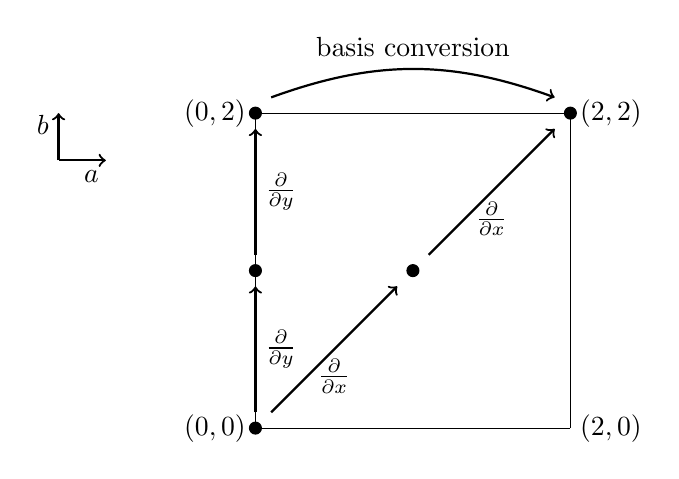
\begin{tikzpicture} 
% Box/square (4x4)
\draw[black,solid,ultra thin] (0,0)--(0,4);
\draw[black,solid,ultra thin] (0,0)--(4,0);
\draw[black,solid,ultra thin] (4,0)--(4,4);
\draw[black,solid,ultra thin] (0,4)--(4,4);
% Dots
\draw[black,fill=black] (0,0) circle (.5ex);
\draw[black,fill=black] (2,2) circle (.5ex);
\draw[black,fill=black] (4,4) circle (.5ex);
\draw[black,fill=black] (0,2) circle (.5ex);
\draw[black,fill=black] (0,4) circle (.5ex);
% Arrows
\draw[black,thick,->] (0.2,0.2)--(1.8,1.8);
\draw[black,thick,->] (2.2,2.2)--(3.8,3.8);
\draw[black,thick,->] (0,0.2)--(0,1.8);
\draw[black,thick,->] (0,2.2)--(0,3.8);
\draw [black,thick,->] (0.2,4.2) to [out=20,in=160] (3.8,4.2);
% Node (parameter) labels
\draw[] (0,0) node[anchor=east] {$(0,0)$};
\draw[] (0,4) node[anchor=east] {$(0,2)$};
\draw[] (4,0) node[anchor=west] {$(2,0)$};
\draw[] (4,4) node[anchor=west] {$(2,2)$};
% Arrow labels
\draw[] (1,1) node[anchor=north] {$\tfrac{\partial}{\partial x}$};
\draw[] (3,3) node[anchor=north] {$\tfrac{\partial}{\partial x}$};
\draw[] (0,1) node[anchor=west] {$\tfrac{\partial}{\partial y}$};
\draw[] (0,3) node[anchor=west] {$\tfrac{\partial}{\partial y}$};
% The key and headings
\draw[black,thick,->] (-2.5,3.4)--(-2.5,4);
\draw[black,thick,->] (-2.5,3.4)--(-1.9,3.4);
\draw[] (-2.3,3.2) node[anchor=west] {$a$};
\draw[] (-2.7,3.6) node[anchor=south] {$b$};
\draw[] (2,4.6) node[anchor=south] {basis conversion};
\end{tikzpicture} 
\caption{The Laplace operator acting on vectors of $\hdop_{n,k}=\hdop_{n,k}^{(0,0)}$ coefficients has a sparse matrix representation if the range is represented as vectors of $\smash{\jac^{(2,2)}_{n,k}}$ coefficients. Here, the arrows indicate that the corresponding operation has a sparse matrix representation when the domain is $\smash{\hdopnkab}$ coefficients, where $(a,b)$ is at the tail of the arrow, and the range is $\smash{\hdop_{n,k}^{(\tilde{a},\tilde{b})}}$ coefficients, where $(\tilde{a},\tilde{b})$ is at the head of the arrow. %For example, $\smash{\frac{\partial}{\partial x}}$ has a sparse matrix representation when the domain is represented in $\smash{\hdop_{n,k}^{(0,0,0)}}$ (resp.~$\smash{\hdop_{n,k}^{(1,0,1)}}$) and the range in $\smash{\hdop_{n,k}^{(1,0,1)}}$ (resp.~$\smash{\hdop_{n,k}^{(2,0,2)}}$).
}
\label{fig:Laplace} 
\end{figure}

Denote the weighted OPs by
\begin{align*}
\bigWab(x,y) := \Wab(x,y) \bighdopab(x,y).
\end{align*}

Recall that a function $f(x,y)$ defined on $\Omega$ is approximated by its expansion $f(x,y) = \bighdopab(x,y)^\top \mathbf{f}$. Recall also that $\Wab(x,y) := \genjacw^{(a,b)}(x) \: \jacw^{(b)}(\frac{y}{\rho(x)})$, where $\rho(x) := (1-x^2)^\half$, $\genjacw^{(a,b)}(x) := x^a \: (1-x^2)^b$ and $\jacw^{(b)}(y) := (1-y^2)^b$ for the half-disk case.

\begin{definition}\label{def:differentialoperators}
Define the operator matrices $D_x^{(a,b)}, \: D_y^{(a,b)}, \: W_x^{(a,b)}, \: W_y^{(a,b)}$ according to:
\begin{align*}
{\partial f \over \partial x}&= \bighdop^{(a+1,b+1)}(x,y)^\top \: D_x^{(a,b)} \: \mathbf{f}, \\
{\partial f \over \partial y} &= \bighdop^{(a,b+1)}(x,y)^\top \: D_y^{(a,b)} \: \mathbf{f}, \\
{\partial \over \partial x}[\Wab(x,y) \: f(x,y)] &= \bigW^{(a-1,b-1)}(x,y)^\top \: W_x^{(a,b)} \: \mathbf{f}, \\
{\partial \over \partial y}[\Wab(x,y) \: f(x,y)] &= \bigW^{(a,b-1)}(x,y)^\top \: W_y^{(a,b)} \: \mathbf{f}.
\end{align*}
\end{definition}

The incrementing and decrementing of parameters as seen here is analogous to other well known orthogonal polynomial families' derivatives, for example the Jacobi polynomials on the interval, as seen in the DLMF \cite[(18.9.3)]{DLMF}, and on the triangle \cite{olver2018recurrence}.

\begin{theorem}\label{theorem:sparsityofdifferentialoperators}
The operator matrices $D_x^{(a,b)}, \: D_y^{(a,b)}, \: W_x^{(a,b)}, \: W_y^{(a,b)}$ from Definition \ref{def:differentialoperators} are sparse, with banded-block-banded structure. More specifically:
\begin{itemize}
	\item $D_x^{(a,b)}$ has  block-bandwidths $(-1,2)$, and sub-block-bandwidths $(0, 2)$.
  	\item $D_y^{(a,b)}$ has  block-bandwidths $(-1,1)$, and sub-block-bandwidths $(-1,1)$.
	\item $W_x^{(a,b)}$ has  block-bandwidths $(2,-1)$, and sub-block-bandwidths $(2, 0)$.
  	\item $W_y^{(a,b)}$ has  block-bandwidths $(1,-1)$, and sub-block-bandwidths $(1,-1)$.
\end{itemize}
\end{theorem}

\begin{proof}
First, note that:
\begin{align}
	\genjacw^{(a,b) \: \prime}(x) &= a \: \genjacw^{(a-1,b)}(x) - 2b \: \genjacw^{(a+1,b-1)}(x), \label{eqn:derivativeofweightgenjac} \\
	\jacw^{(b) \: \prime}(y) &= - 2b \: y \: \jacw^{(b-1)}(y), \label{eqn:derivativeofweightjac}
\end{align}

We proceed with the case for the operator $D_y^{(a,b)}$ for partial differentiation by $y$. Since $\{\hdop^{(a, b+1)}_{m,j}\}$ for $m = 0,\dots,n-1$, $j = 0,\dots,m$ is an orthogonal basis for any degree $n-1$ polynomial, we can expand $\pddy \hdopnkab = \sum_{m=0}^{n-1} \sum_{j=0}^m c_{m,j}^y \: \hdop^{(a, b+1)}_{m,j}$. The coefficients of the expansion are then the entries of the relevant operator matrix. We can use an integration-by-parts argument to show that the only non-zero coefficient of this expansion is when $m = n-1$, $j = k-1$. First, note that
\begin{align*}
	c_{m,j}^y = {\ip<\pddy \hdopnkab, \hdop^{(a, b+1)}_{m,j} >_{W^{(a, b+1)}}}{\norm{\hdop^{(a, b+1)}_{m,j}}^{-2}_{W^{(a, b+1)}}}.
\end{align*}
Then, using the change of variable $t = \frac{y}{\rho(x)}$, we have that
\begin{align*}
	\ip<\pddy \hdopnkab, \hdop^{(a, b+1)}_{m,j} >_{W^{(a, b+1)}} &= \normgenjac^{(a, b+1)} \: \ip< \genjacnmk^{(a,b+k+\half)}, \rho(x)^{k+j} \: \genjacmmj^{(a,b+1+j+\half)} >_{\genjacw^{(a,b+1)}} \\
	&\quad \quad \quad \quad \quad \quad \cdot \: \normjac^{(b+1)} \: \ip< \jac_k^{(b,b) \: \prime}, \: \jac_{j}^{(b+1,b+1)} >_{\jacw^{(b+1)}} \\
	&= \normgenjac^{(a, b+1+\half(k+j))} \: \ip< \genjacnmk^{(a,b+k+\half)}, \genjacmmj^{(a,b+1+j+\half)} >_{\genjacw^{(a,b+1+\half(k+j))}} \\
		&\quad \quad \quad \quad \quad \quad \cdot \: \normjac^{(b+1)} \: \ip< \jac_k^{(b,b) \: \prime}, \: \jac_{j}^{(b+1,b+1)} >_{\jacw^{(b+1)}}.
\end{align*}
Now, using (\ref{eqn:derivativeofweightjac}), integration-by-parts, and noting that the weight $\jacw^{(b)}$ is a polynomial of degree $2b$ and vanishes at the limits of the integral for positive parameter $b$, we have that
\begin{align*}
	\normjac^{(b+1)} \: \ip< \jac_k^{(b,b) \: \prime}, \: \jac_{j}^{(b+1,b+1)} >_{\jacw^{(b+1)}} &= \int_{-1}^1 \: \jac_k^{(b,b) \: \prime}(y) \: \jac_{j}^{(b+1,b+1)}(y) \: \jacw^{(b+1)}(y) \: \D y \\
	&= - \int_{-1}^1 \: \jac_k^{(b,b)}(y) \: \ddy [\jacw^{(b+1)}(y) \: \jac_{j}^{(b+1,b+1)}(y)] \: \D y \\
	&= - \int_{-1}^1 \: \jac_k^{(b,b)} \: [ \jac_{j}^{(b+1,b+1) \: \prime} \: \jacw^{(b+1)} - 2 b \: y \: \jac_{j}^{(b+1,b+1)} \:\jacw^{(b)} ] \: \D y \\
	&= - \: \normjac^{(b)} \: \ip< \jac_k^{(b,b)}, \: \jacw^{(1)} \: \jac_{j}^{(b+1,b+1) \: \prime} -2b \:y \: \jac_{j}^{(b+1,b+1)} >_{\jacw^{(b)}}
\end{align*}
which is zero for $j < k-1$. Further,
\begin{align*}
	\ip< \genjacnmk^{(a,b+k+\half)}, \genjac_{m+1-k}^{(a,b+k+\half)} >_{\genjacw^{(a,b+k+\half)}} = \delta_{n,m+1},
\end{align*}
showing that the only possible non-zero coefficient is when $m=n-1, j=k-1$. Finally,
\begin{align*}
	c_{n-1,k-1}^y &= \ip< \jac_k^{(b,b) \: \prime}, \: \jac_{k-1}^{(b+1,b+1)} >_{\jacw^{(b+1)}}.
\end{align*}

We next consider the case for the operator $D_x^{(a,b)}$ for partial differentiation by $x$. Since $\{\hdop^{(a+1, b+1)}_{m,j}\}$ for $m = 0,\dots,n-1$, $j = 0,\dots,m$ is an orthogonal basis for any degree $n-1$ polynomial, we can expand $\pddx \hdopnkab = \sum_{m=0}^{n-1} \sum_{j=0}^m c_{m,j}^x \: \hdop^{(a+1, b+1)}_{m,j}$. The coefficients of the expansion are then the entries of the relevant operator matrix. As before, we can use an integration-by-parts argument to show that the only non-zero coefficients of this expansion are when $m = n-1, n-2$, $j = k, k-1, k-2$ and $0 \le j \le m$. First, note that
\begin{align*}
	c_{m,j}^x = {\ip<\pddx \hdopnkab, \hdop^{(a+1, b+1)}_{m,j} >_{W^{(a+1, b+1)}}}{\norm{\hdop^{(a+1, b+1)}_{m,j}}^{-2}_{W^{(a+1, b+1)}}}.
\end{align*}
Second, note that
\begin{align}
	\rho'(x) = -x \: \rho(x)^{-1}. \label{eqn:rhoderivative}
\end{align}
Now, using the change of variable $t= \frac{y}{\rho(x)}$ and (\ref{eqn:rhoderivative}), we have that
\begin{align*}
	&\ip<\pddx \hdopnkab, \hdop^{(a+1, b+1)}_{m,j} >_{W^{(a+1, b+1)}} \nonumber \\ 
	&= \normgenjac^{(a, b+\half)} \: \normjac^{(b+1)} \: \Big\{ \ip< x \: \genjacnmk^{(a, b+k+\half) \: \prime} (x), \: \rho(x)^{k+j+2} \: \genjacmmj^{(a+1, b+1+j+\half)} >_{\genjacw^{(a, b+\half)}} \\ 
	&\quad \quad \quad \quad \quad \quad \quad \quad \quad \quad \quad \quad \cdot \: \ip< \jac_k^{(b,b)}, \: \jac_j^{(b+1,b+1)} >_{\jacw^{(b+1)}}  \nonumber \\ 
	& \quad - k \: \ip< x^2 \: \genjacnmk^{(a, b+k+\half)}(x), \: \rho(x)^{k+j} \: \genjacmmj^{(a+1, b+1+j+\half)} >_{\genjacw^{(a, b+\half)}} 
		\: \ip< \jac_k^{(b,b)}, \: \jac_j^{(b+1,b+1)} >_{\jacw^{(b+1)}}  \nonumber \\ 
	& \quad + \: \ip< x^2 \: \genjacnmk^{(a, b+k+\half)}(x), \: \rho(x)^{k+j} \: \genjacmmj^{(a+1, b+1+j+\half)} >_{\genjacw^{(a, b+\half)}} 
		\: \ip< y \: \jac_k^{(b,b) \: \prime} (y), \: \jac_j^{(b+1,b+1)} >_{\jacw^{(b+1)}} \Big\}
\end{align*}

We can see  from each term's second factor that the above is zero for $j < k-2$. Now, using (\ref{eqn:derivativeofweightgenjac}), integration-by-parts, and noting that the weight $\genjacw^{(a,b)}$ is a polynomial degree $a+2b$ and vanishes at the limits of the integral for positive parameters $a,b$, we have that
\begin{align*}
	&\normgenjac^{(a, b+\half)} \: \ip< x \: \genjacnmk^{(a, b+k+\half) \: \prime}, \: \rho(x)^{k+j+2} \: \genjacmmj^{(a+1, b+1+j+\half)} >_{\genjacw^{(a, b+\half)}}  \\
	&= \int_0^1 \: \genjacnmk^{(a, b+k+\half) \: \prime} \: \genjacmmj^{(a+1, b+1+j+\half)} \: \genjacw^{(a+1, b+1+\half(k+j+1))} \: \D x \\
	&= - \int_0^1 \: \genjacnmk^{(a, b+k+\half)} \: \ddx \Big[ \genjacmmj^{(a+1, b+1+j+\half)} \: \genjacw^{(a+1, b+1+\half(k+j+1))} \Big] \: \D x \\
	&= - \int_0^1 \: \genjacnmk^{(a, b+k+\half)} \: \Big\{ \genjacw^{(a+1, b+1+\half(k+j+1))} \: \genjacmmj^{(a+1, b+1+j+\half) \: \prime} \\
	&\quad \quad \quad \quad \quad \quad \quad \quad \quad \quad + (a+1) \: \genjacw^{(a, b+1+\half(k+j+1))} \: \genjacmmj^{(a, b+1+j+\half)} \\
	&\quad \quad \quad \quad \quad \quad \quad \quad \quad \quad -2(b+1+\half(k+j+1)) \: \genjacw^{(a+2, b+\half(k+j+1))} \: \genjacmmj^{(a, b+1+j+\half)} \Big\} \: \D x \\
	&= - \: \normgenjac^{(a,b+k+\half)} \:  \Big\{ \ip<\genjacnmk^{(a, b+k+\half)}, \: \genjacw^{(1, 1+\half(j-k))} \: \genjacmmj^{(a+1, b+1+j+\half) \: \prime}>_{\genjacw^{(a, b+k+\half)}} \\
		&\quad \quad \quad + \ip<\genjacnmk^{(a, b+k+\half)}, \: (a+1) \: \genjacw^{(0,1+\half(j-k))} \genjacmmj^{(a, b+1+j+\half)} >_{\genjacw^{(a, b+k+\half)}} \\
		&\quad \quad \quad - \ip<\genjacnmk^{(a, b+k+\half)}, \: 2(b+1+\half(k+j+1)) \: \genjacw^{(2, \half(j-k))} \: \genjacmmj^{(a, b+1+j+\half)} >_{\genjacw^{(a, b+k+\half)}} \Big\}
\end{align*}
which is zero for $m < n - 2$, and further that
\begin{align*}
	&\normgenjac^{(a, b+\half)} \: \ip< x^2 \: \genjacnmk^{(a, b+k+\half)}(x), \: \rho(x)^{k+j} \: \genjacmmj^{(a+1, b+1+j+\half)} >_{\genjacw^{(a, b+\half)}} \\
	&= \normgenjac^{(a, b+k+\half)} \: \ip< \genjacnmk^{(a, b+k+\half)}(x), \: \genjacw^{(2, \half(j-k))} \: \genjacmmj^{(a+1, b+1+j+\half)} >_{\genjacw^{(a, b+k+\half)}}
\end{align*}
which is also zero for $m < n - 2$.

We can gain the non-zero entries of the weighted differential operators similarly, by noting that
\begin{align}
	\pddx \Wab(x,y) &= a W^{(a-1, b)}(x,y) - 2bW^{(a+1, b-1)}(x,y) \label{eqn:weightderivativex} \\
	\pddy \Wab(x,y) &= -2b \: y \: W^{(a, b-1)}(x,y) \label{eqn:weightderivativey}
\end{align}
and also that
\begin{align*}
	\ip< \Wab \hdopnkab, W^{(\tilde{a},\tilde{b})} \hdopmj^{(\tilde{a},\tilde{b})} >_{W^{(-\tilde{a},-\tilde{b})}} = \ip< \hdopnkab, \hdopmj^{(\tilde{a},\tilde{b})} >_\Wab.
\end{align*}

\end{proof}

There exist conversion matrix operators that increment/decrement the parameters, transforming the OPs from one (weighted or non-weighted) parameter space to another. 

\begin{definition}\label{def:parametertransformationoperators}
Define the operator matrices $T^{(a,b)\to(a+1,b)}$, $T^{(a,b)\to(a,b+1)}$ and $T^{(a,b)\to(a+1,b+1)}$ for conversion between non-weighted spaces, and $T_W^{(a,b)\to(a-1,b)}$, $T_W^{(a,b)\to(a,b-1)}$ and $T_W^{(a,b)\to(a-1,b-1)}$ for conversion between weighted spaces, according to:
\begin{align*}
	\bighdop^{(a,b)}(x,y) &= \Big(T^{(a,b)\to(a+1,b)} \Big)^\top \: \bighdop^{(a+1,b)}(x,y) \\
	\bighdop^{(a,b)}(x,y) &= \Big(T^{(a,b)\to(a,b+1)} \Big)^\top \: \bighdop^{(a,b+1)}(x,y) \\
	\bighdop^{(a,b)}(x,y) &= \Big(T^{(a,b)\to(a+1,b+1)} \Big)^\top \: \bighdop^{(a+1,b+1)}(x,y) \\
	\bigW^{(a,b)}(x,y) &= \Big(T_W^{(a,b)\to(a-1,b)} \Big)^\top \: \bigW^{(a-1,b)}(x,y) \\
	\bigW^{(a,b)}(x,y) &= \Big(T_W^{(a,b)\to(a,b-1)} \Big)^\top \: \bigW^{(a,b-1)}(x,y) \\
	\bigW^{(a,b)}(x,y) &= \Big(T_W^{(a,b)\to(a-1,b-1)} \Big)^\top \: \bigW^{(a-1,b-1)}(x,y).
\end{align*}
\end{definition}

\begin{lemma}\label{lemma:sparsityofparametertransformationoperators}
The operator matrices in Definition \ref{def:parametertransformationoperators} are sparse, with banded-block-banded structure. More specifically:
\begin{itemize}
	\item $T^{(a,b)\to(a+1,b)}$ has block-bandwidth $(0,1)$, with diagonal blocks.
  	\item $T^{(a,b)\to(a,b+1)}$, $T^{(a,b)\to(a+1,b+1)}$ have block-bandwidth $(0,3)$ and sub-block-bandwidth $(0,2)$.
	\item $T_W^{(a,b)\to(a-1,b)}$ has block-bandwidth  $(1,0)$ with diagonal blocks.
  	\item $T_W^{(a,b)\to(a,b-1)}$, $T_W^{(a,b)\to(a-1,b-1)}$ have block-bandwidth $(3,0)$ and sub-block-bandwidth $(2,0)$.
\end{itemize}
\end{lemma}

\begin{proof}
We proceed with the case for the non-weighted operators $T^{(a,b)\to(a+\lambda,b+\mu)}$, where $\lambda, \mu \in \{0,1\}$. Since $\{\hdop^{(a+\lambda, b+\mu)}_{m,j}\}$ for $m = 0,\dots,n$, $j = 0,\dots,m$ is an orthogonal basis for any degree $n$ polynomial, we can expand $\hdopnkab = \sum_{m=0}^{n} \sum_{j=0}^m c_{m,j} \: \hdop^{(a+\lambda, b+\mu)}_{m,j}$. The coefficients of the expansion are then the entries of the relevant operator matrix. We will see that the only non-zero coefficients are for $m \ge n - \lambda - 2\mu $, $j \ge k-2\mu$ and $0 \le j \le m$. First, note that
\begin{align*}
	c_{m,j} = {\ip< \hdopnkab, \hdop^{(a+\lambda, b+\mu)}_{m,j} >_{W^{(a+\lambda, b+\mu)}}}{\norm{\hdop^{(a+\lambda, b+\mu)}_{m,j}}^{-2}_{W^{(a+\lambda, b+\mu)}}}.
\end{align*}
Then, using the change of variable $t = \frac{y}{\rho(x)}$, we have that
\begin{align*}
	&\ip< \hdopnkab, \hdop^{(a+\lambda, b+\mu)}_{m,j} >_{W^{(a+\lambda, b+\mu)}} \\
	&\quad = \normgenjac^{(a+\lambda, b+\mu)} \: \ip< \genjacnmk^{(a,b+k+\half)}, \rho(x)^{k+j+1} \: \genjacmmj^{(a+\lambda,b+\mu+j+\half)} >_{\genjacw^{(a+\lambda,b+\mu)}} \\ 
	&\quad \quad \quad \cdot \: \normjac^{(b+\mu)} \: \ip< \jac_k^{(b,b)}, \: \jac_{j}^{(b+\mu,b+\mu)} >_{\jacw^{(b+\mu)}} \\
	&\quad= \normgenjac^{(a, b+k+\half)} \: \ip< \genjacnmk^{(a,b+k+\half)}, \genjacw^{(\lambda, \: \mu+\half(j-k))} \: \genjacmmj^{(a+\lambda,b+\mu+j+\half)} >_{\genjacw^{(a,b+k+\half)}} \\
	&\quad \quad \quad \cdot \: \normjac^{(b)} \: \ip< \jac_k^{(b,b)}, \: \jacw^{(\mu)} \: \jac_{j}^{(b+\mu,b+\mu)} >_{\jacw^{(b)}}
\end{align*}
Since $\jacw^{(\mu)}$ is a polynomial degree $2\mu$, we have that the above is then zero for $j < k-2\mu$. Further, since $\genjacw^{(\lambda, \: \mu+\half(j-k))}$ is a polynomial of degree $\lambda + 2\mu + j - k$, we have that the above is zero for $m-j < n-k - (\lambda + 2\mu + j - k) \iff m < n - \lambda - 2\mu$.

The sparsity argument for the weighted parameter transformation operators follows similarly.
\end{proof}

\begin{figure}[t]
	\begin{subfigure}{0.32\textwidth}
	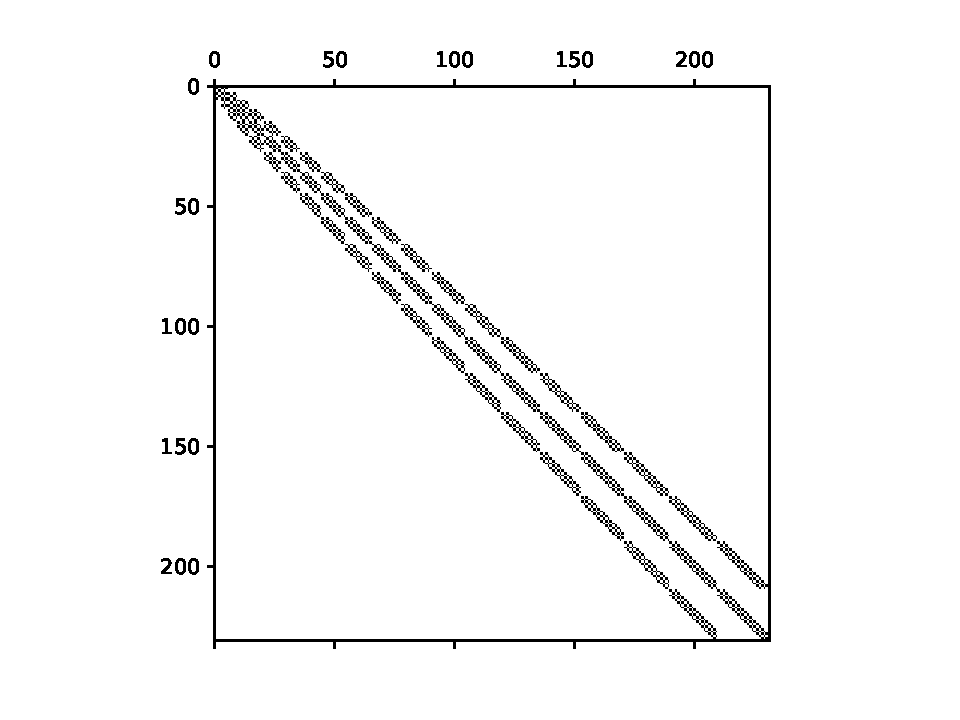
\includegraphics[scale=0.35]{sparsityoflaplacian-w11}
        \centering
	\end{subfigure}
	\begin{subfigure}{0.32\textwidth}
	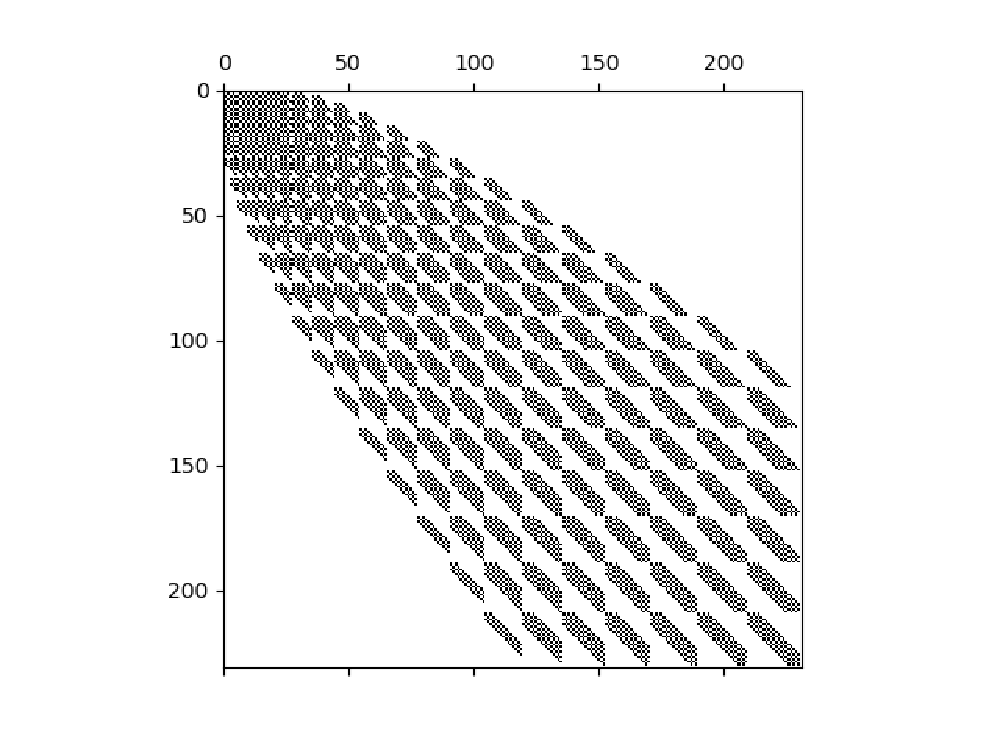
\includegraphics[scale=0.35]{sparsityofhelmholtz}
        \centering
	\end{subfigure}
	\begin{subfigure}{0.32\textwidth}
	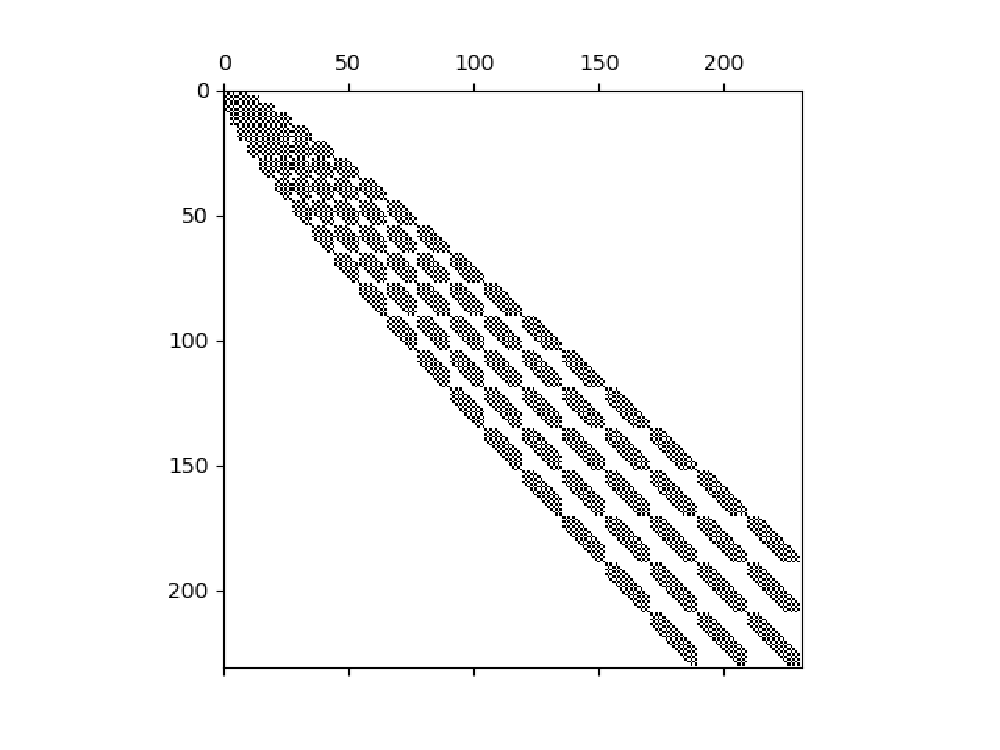
\includegraphics[scale=0.35]{sparsityofbiharmonic}
        \centering
	\end{subfigure}
    	\caption{"Spy" plots of (differential) operator matrices, showing their sparsity. Left: the Laplace operator $\laplacewii$. Centre: the weighted variable coefficient Helmholtz operator $\laplacewii + k^2 \: T^{(0,0)\to(1,1)} \: V({J_x^{(0,0)}}^\top, {J_y^{(0,0)}}^\top) \: T_W^{(1,1)\to(0,0)}$ for $v(x,y) = 1 - (3(x-1)^2 + 5y^2)$ and $k = 200$. Right: the biharmonic operator $\biharmonic$.}
        \label{fig:sparsity}
        \centering
\end{figure}

General linear partial differential operators with polynomial variable coefficients can be constructed by composing the sparse representations for partial derivatives, conversion between bases, and Jacobi operators. As a canonical example, we can obtain the matrix operator for the Laplacian \(\Delta\), that will take us from coefficients for expansion in the weighted space
$$
\bigWii(x,y) = \Wii(x,y) \: \bighdopii(x,y)
$$
to coefficients in the non-weighted space $\bighdopii(x,y)$. Note that this construction will ensure the imposition of the Dirichlet zero boundary conditions on $\Omega$. The matrix operator for the Laplacian we denote $\laplacewii$ acting on the coefficients vector is then given by
\begin{align*}
    \laplacewii := D_x^{(0,0)} \: W_x^{(1,1)} + T^{(0,1)\to(1,1)} \: D_y^{(0,0)} \: T_W^{(1,0)\to(0,0)} \: W_y^{(1,1)}.
\end{align*}
Importantly, this operator will have banded-block-banded structure, and hence will be sparse, as seen in Figure \ref{fig:sparsity}.

Another important example is the Biharmonic operator $\Delta^2$, where we assume zero Dirichlet and Neumann conditions. To construct this operator, we first note that we can obtain the matrix operator for the Laplacian $\Delta$ that will take us from coefficients for expansion in the space $\bighdopoo(x,y)$ to coefficients in the space $\bighdop^{(2,2)}(x,y)$. We denote this matrix operator that acts on the coefficients vector as $\laplaceoo$, and is given by
\begin{align*}
    \laplaceoo := D_x^{(1,1)} \: D_x^{(0,0)} + T^{(1,2)\to(2,2)} \: D_y^{(1,1)} \: T^{(0,1)\to(1,1)} \: D_y^{(0,0)}.
\end{align*}
Further, we can represent the Laplacian as a map from coefficients in the space $\bigW^{(2,2)}$ to coefficients in the space $\bighdopoo$. Note that a function expanded in the $\bigW^{(2,2)}$ basis will satisfy both zero Dirichlet and Neumann boundary conditions on $\Omega$. We denote this matrix operator as $\laplacewtt$, and is given by
\begin{align*}
	\laplacewtt := W_x^{(1,1)} \: W_x^{(2,2)} + T_W^{(1,0)\to(0,0)} \: W_y^{(1,1)} \: T_W^{(2,1)\to(1,1)} \: W_y^{(2,2)}.
\end{align*}
We can then construct a matrix operator for $\Delta^2$ that will take coefficients in the space $\bigW^{(2,2)}$ to coefficients in the space $\bighdop^{(2,2)}$. Note that any function expanded in the $\bigW^{(2,2)}$ basis will satisfy both zero Dirichlet and zero Neumann boundary conditions on $\Omega$. The matrix operator for the Biharmonic operator is then given by
\begin{align*}
	\biharmonic = \laplaceoo \: \laplacewtt.
\end{align*}
The sparsity and structure of this biharmonic operator is seen in Figure \ref{fig:sparsity}.



\section{Computational aspects}\label{Section:Computation}

In this section we discuss how to take advantage of the proposed basis and sparsity structure in partial differential operators in practical computational applications. 

\subsection{Constructing $\genjac_n^{(a,b)}(x)$}

To obtain the recurrence coefficients for the $\{\genjac_n^{(a,b)}\}$ OPs in (\ref{eqn:Hrecurrence}), we use a variant of the Stieltjes procedure \cite{gautschi1982generating} where the polynomials are expressed as Chebyshev polynomial expansions and the inner products are calculated via Clenshaw--Curtis quadrature. This has the benefit that it is easier to incorporate high-precision arithmetic, which we use to overcome ill-conditioning present when $b$ is large, as required for large $n$ in \eqref{eq:diskpolys}. The ApproxFun.jl \cite{ApproxFun} package gives a convenient way to manipulate Chebyshev and Jacobi expansions, which we use to calculate the inner products and norms in this algorithm, utilising the {\tt BigFloat} type to handle high-precision calculations.

\noindent{\bf Remark}: 
This is the most expensive part of the current calculation, but note that we can reuse this computation for multiple partial differential equations. Efficient construction of OPs with large parameters in the weights is an important topic, but one tangential to the proposed scheme. 

\subsection{Quadrature rules}

In this section we construct a quadrature rule exact for polynomials in $\Omega$ that can be used to expand functions in $\hdopnkab(x,y)$. 

\begin{theorem}

Denote the  Gauss quadrature nodes and weight on \([0,1]\) with weight \(s^a \: (1-s^2)^{b+\half}\) as $(s_k,w_k^{(s)})$ , and
 on \([-1,1]\) with weight \((1-t^2)^b\) as $(t_k,w_k^{(t)})$. Define
\begin{align*}
x_{i+(k-1)N} &:= s_k, \quad i,k = 1,\dots,N, \\
y_{l+(i-1)N} &:= (1-s_l^2)^\half \: t_l, \quad i,l = 1,\dots,N, \\
w_{l+(k-1)N} &:= w_k^{(s)} w_l^{(t)}, \quad k,l = 1,\dots,N.
\end{align*}
Let $f(x,y)$ be a polynomial on $\Omega$. The quadrature rule is then
$$
\iint_\Omega f(x,y) \: \Wab(x,y) \: \D A \approx \half \sum_{j=1}^{N^2} w_j \: \big[ f(x_j, y_j) + f(x_j, -y_j) \big],
$$
and the quadrature rule is exact if $x \mapsto f(x,y)$ for fixed $y$ is an at most degree $N$ polynomial and $y \mapsto f(x,y)$ for fixed $x$ is an at most degree $2N-1$ polynomial.
\end{theorem}

\begin{proof}
We will use the substitution that
\begin{align*}
	x &= s, \quad y = \rho(s) \: t.
\end{align*}
First, note that, for $(x,y) \in \Omega$,
\begin{align*}
	W^{(a,b)}(x,y) &= \genjacw^{(a,b)}(x) \: \jacw^{(b)}\fpr(\frac{y}{\rho(x)}) \\
	&= \genjacw^{(a,b)}(s) \: \jacw^{(b)}(t) \\
	&= s^a \: \rho(s)^{2b} \: (1-t^2)^b \\
	&=: V^{(a,b)}(s,t), \quad \text{for } (s,t) \in [0,1] \times [-1,1].
\end{align*}

Let $f : \Omega \to \R$. Define the functions $f_e, f_o : \Omega \to \R$ by 
\begin{align*}
	f_e(x,y) &:= \half \Big(f(x, y) + f(x, -y)\Big), \quad \forall (x,y) \in \Omega\\
	f_o(x,y) &:= \half \Big(f(x, y) - f(x, -y)\Big), \quad \forall (x,y) \in \Omega
\end{align*}
so that $y \mapsto f_e(x,y)$ for fixed $x$ is an even function, and $y \mapsto f_o(x,y)$ for fixed $x$ is an odd function. Note that if $f$ is a polynomial, then $f_e(s, \rho(s)t)$ is a polynomial in $s \in [\alpha,\beta]$ for fixed $t$. 

Now, we have that
\begin{align*}
	\iint_\Omega f_e(x,y) \: \Wab(x,y) \: \D y \: \D x &= \int_\alpha^\beta \int_\gamma^\delta f_e\big(s,\rho(s) t\big) \: V^{(a,b)}(s,t) \: \rho(s) \: \D t \: \D s \\
	&= \int_\alpha^\beta  \genjacw^{(a,b+\half)}(s) \: \Big( \int_\gamma^\delta f_e\big(s,\rho(s) t\big) \: \jacw^{(b)}(t) \: \D t \Big) \: \D s \\
	&\approx \int_\alpha^\beta  \genjacw^{(a,b+\half)}(s) \: \sum_{k=1}^N \Big( w_k^{(t)} f_e\big(s,\rho(s) t_k\big) \Big) \: \D s \quad (\star) \\
	&\approx \sum_{k=1}^N \Bigg( w_k^{(s)} \: \sum_{l=1}^N \Big( w_l^{(t)} f_e\big(s_k,\rho(s_k) t_l\big) \Big) \Bigg) \quad (\star \star) \\
	&= \sum_{j=1}^{N^2}  w_j \: f_e(x_j, y_j),
\end{align*}
where we achieve equality at $(\star)$ if $y \mapsto f_e(x,y)$ for fixed $x$ is a polynomial of degree at most $2N-1$ and we achieve equality at $(\star \star)$ if also $x \mapsto f_e(x,y)$ for fixed $y$ is a polynomial of degree at most $N$. 

Next, note that 
\begin{align*}
	\iint_\Omega f_o(x,y) \: \Wab(x,y) \: \D y \: \D x &= \int_\alpha^\beta \int_\gamma^\delta f_o\big(s,\rho(s) t\big) \: V^{(a,b)}(s,t) \: \rho(s) \: \D t \: \D s \\
	&= \int_\alpha^\beta  \genjacw^{(a,b+\half)}(s) \: \Big( \int_\gamma^\delta f_o\big(s,\rho(s) t\big) \: \jacw^{(b)}(t) \: \D t \Big) \: \D s \quad (\dagger) \\
	&= 0
\end{align*}
since the inner integral at $(\dagger)$ over $t$ is zero, due to the symmetry over the domain (i.e. since $\gamma = -\delta$).

Hence,
\begin{align*}
	\iint_\Omega f(x,y) \: \Wab(x,y) \: \D y \: \D x &= \iint_\Omega \Big(f_e(x,y) + f_o(x,y)\Big) \: \Wab(x,y) \: \D y \: \D x \\
	&= \iint_\Omega f_e(x,y) \: \Wab(x,y) \: \D y \: \D x \\
	&\approx \sum_{j=1}^{N^2}  w_j \: f_e(x_j, y_j) \quad (\star),
\end{align*}
where we achieve equality at $(\star)$ if $y \mapsto f(x,y)$ for fixed $x$ is a polynomial of degree at most $2N-1$ and also if $x \mapsto f(x,y)$ for fixed $y$ is a polynomial of degree at most $N$.
\end{proof}


\subsection{Obtaining the coefficients for expansion of a function}

Fix \(a,b \in \R\). Then for any function \(f : \Omega \to \R\) of degree $N$ we can express \(f\) by
\begin{align*}
f(x,y) = \sum_{n=0}^N \bighdop_n^{(a,b)}(x,y)^\top \: \mathbf{f}_n
\end{align*}
where
\begin{align*}
\bighdop_n(x,y) &:= \begin{pmatrix}
		\hdop_{n,0}(x,y) \\
		\vdots \\
		\hdop_{n,n}(x,y)
	\end{pmatrix} \in \R^{n+1} \quad \forall n = 0,1,2,\dots,N,
\end{align*}
and where
\begin{align*}
\mathbf{f}_n &:= \begin{pmatrix}
		f_{n,0} \\
		\vdots \\
		f_{n,n}
	\end{pmatrix} \in \R^{n+1} \quad \forall n = 0,1,2,\dots,N, \quad
f_{n,k} := \frac{\langle f, \: \hdopnk^{(a,b)} \rangle_{W^{(a,b)}}}{\norm{\hdopnk^{(a,b)}}_{W^{(a,b)}}}
\end{align*}

Recall from (\ref{eqn:normhdop}) that $\norm{\hdopnkab}^2_\Wab = \normgenjac^{(a,b+k+\half)} \: \normjac^{(b)}$. Using the quadrature rule detailed in Section 4.2 for the inner product, we can calculate exactly the coefficients $f_{n,k}$: 
\begin{align*}
	f_{n,k} &= \frac{1}{2 \: \normgenjac^{(a,b+k+\half)} \: \normjac^{(b)}} \: \sum_{j=1}^{N^2} w_j \: \big[ f(x_j, y_j) \: \hdopnk^{(a,b)}(x_j, y_j) +f(x_j, -y_j) \: \hdopnk^{(a,b)}(x_j, -y_j) \big].
\end{align*}


\subsection{Calculating non-zero entries of the operator matrices}\label{subsection:Computation-operatormatrices}

The proofs of Theorem \ref{theorem:sparsityofdifferentialoperators} and Lemma \ref{lemma:sparsityofparametertransformationoperators} provide a way to calculate the non-zero entries of the operator matrices given in Definition \ref{def:differentialoperators} and Definition \ref{def:parametertransformationoperators}. We can simply use quadrature to calculate the 1D inner products, which has a complexity of $\bigO(N^3)$. This proves much cheaper computationally than using the 2D quadrature rule to calculate the 2D inner products, which has a complexity of $\bigO(N^4)$. 


%
\section{Examples on the half-disk with zero Dirichlet conditions}\label{Section:Examples}

We now demonstrate how the sparse linear systems constructed as above can be used to efficiently solve PDEs with zero Dirichlet conditions. We consider Poisson, inhomogeneous variable coefficient Helmholtz equation and the Biharmonic equation, demonstrating the versatility of the approach. 

\subsection{Poisson}

% FIGURES
\begin{figure}[t]
	\begin{subfigure}{0.3\textwidth}
	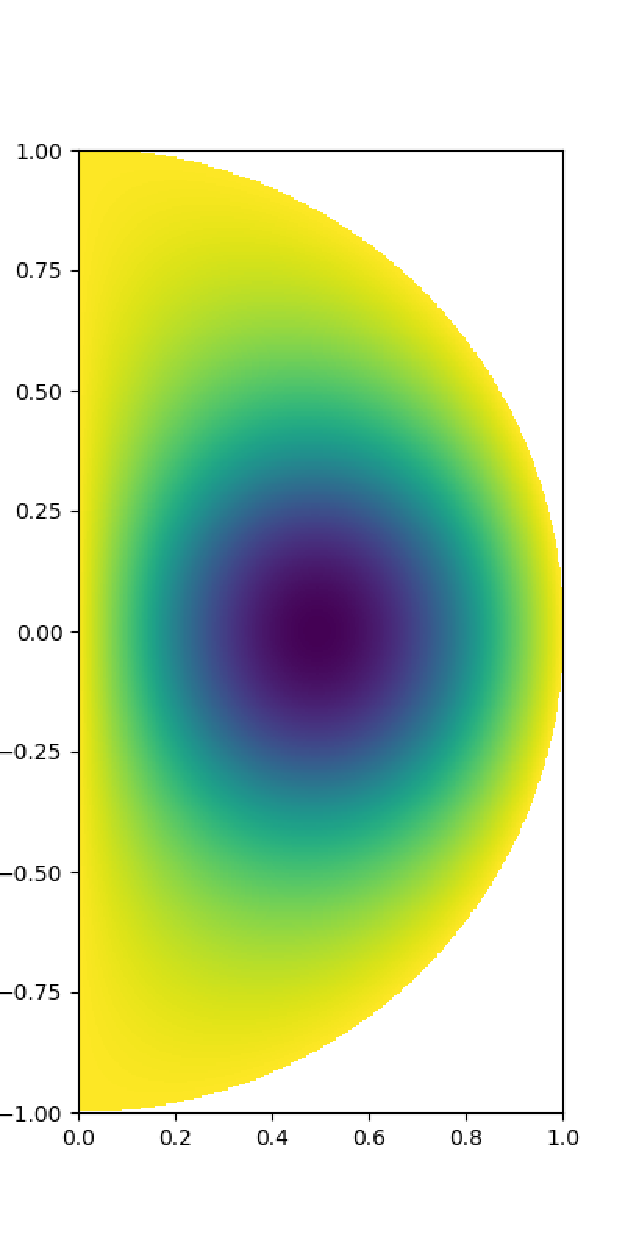
\includegraphics[scale=0.3]{solution-poisson}
	\centering
	%\label{fig:solution-poisson}
	\end{subfigure}
	\begin{subfigure}{0.5\textwidth}
	\centering
	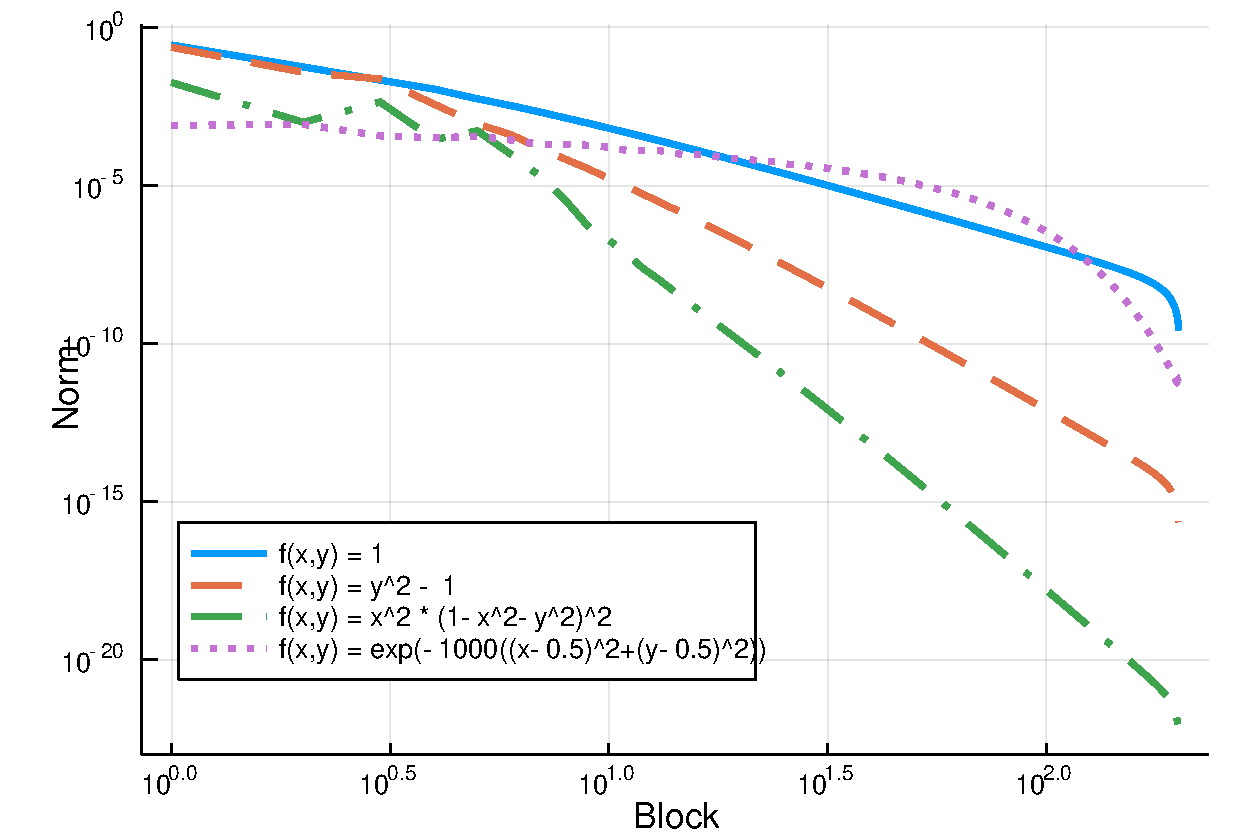
\includegraphics[scale=0.5]{solutionblocknorms-poisson}
        	%\label{fig:solutionblocknorms-poisson}
	\end{subfigure}
	\caption{Left: The computed solution to $\Delta u = f$ with zero boundary conditions with $f(x,y) = 1 + \text{erf}(5(1 - 10((x - 0.5)^2 + y^2)))$. Right: The norms of each block of the computed solution of the Poisson equation with the given right hand side functions. This demonstrates algebraic convergence with the rate dictated by the decay at the corners, with spectral convergence observed when the right-hand side vanishes to all orders.}
	\centering
	\label{fig:poisson}
\end{figure}

\begin{figure}[t]
	\begin{subfigure}{0.3\textwidth}
	\centering
	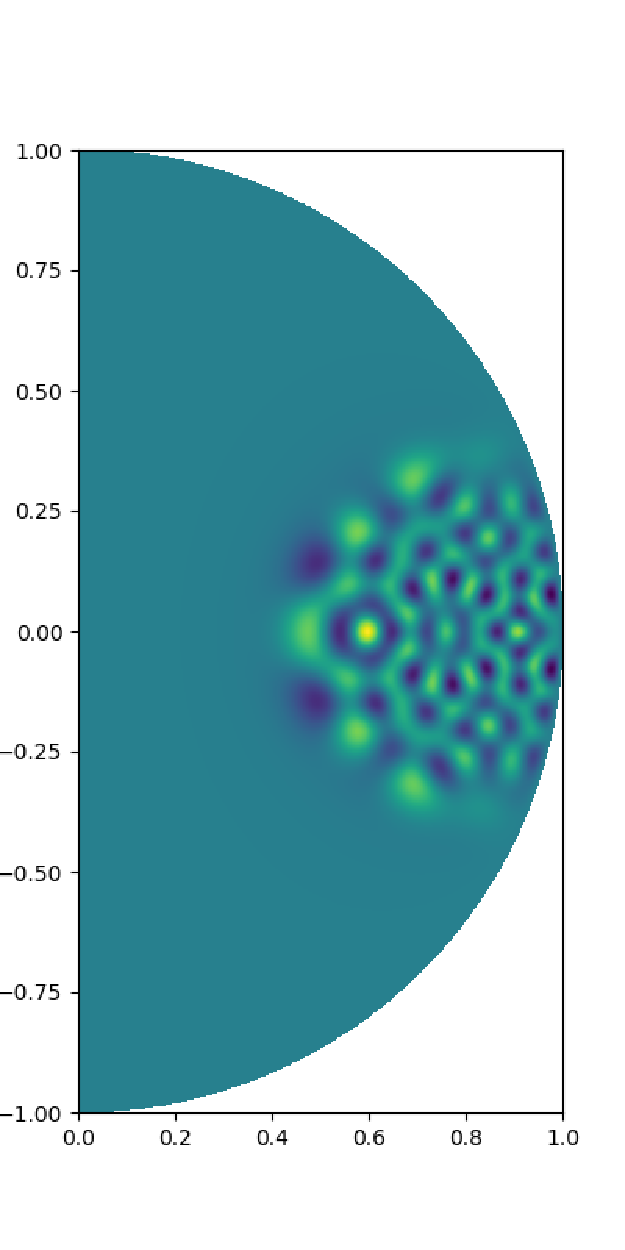
\includegraphics[scale=0.3]{solution-helmholtz-k=100-n=1500}
	%\label{fig:solution-helmholtz}
	\end{subfigure}
	\begin{subfigure}{0.5\textwidth}
	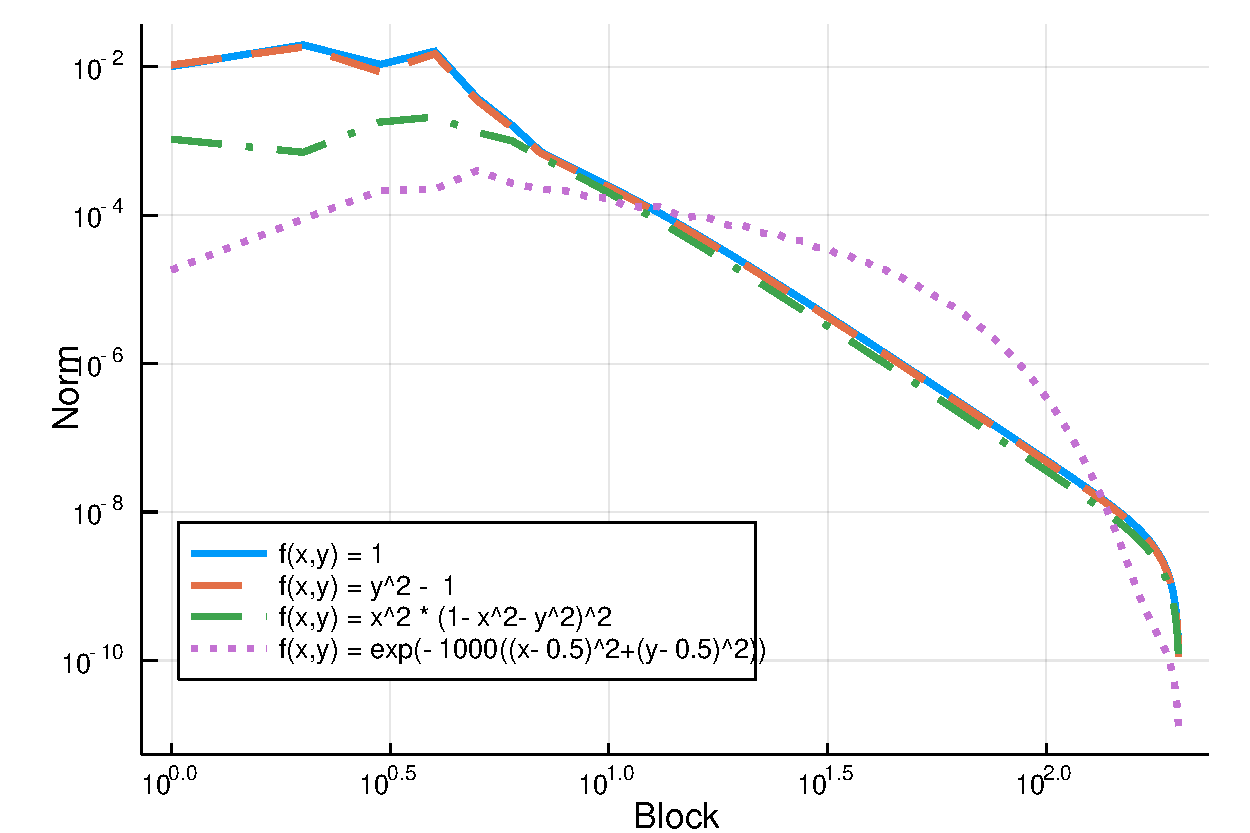
\includegraphics[scale=0.5]{solutionblocknorms-helmholtz-k=20}
	\centering
        	%\label{fig:solutionblocknorms-helmholtz}
	\end{subfigure}
	\caption{Left: The computed solution to $\Delta u + k^2 \: v \: u = f$ with zero boundary conditions with $f(x,y) = x(1-x^2-y^2)e^x$, $v(x,y) = 1 - (3(x-1)^2 + 5y^2)$ and $k = 100$. Right: The norms of each block of the computed solution of the Helmholtz equation with the given right hand side functions, with $k=20$ and $v(x,y) = 1 - (3(x-1)^2 + 5y^2)$.}
	\centering
	\label{fig:helmholtz}
\end{figure}

\begin{figure}[t]
	\begin{subfigure}{0.3\textwidth}
	\centering
	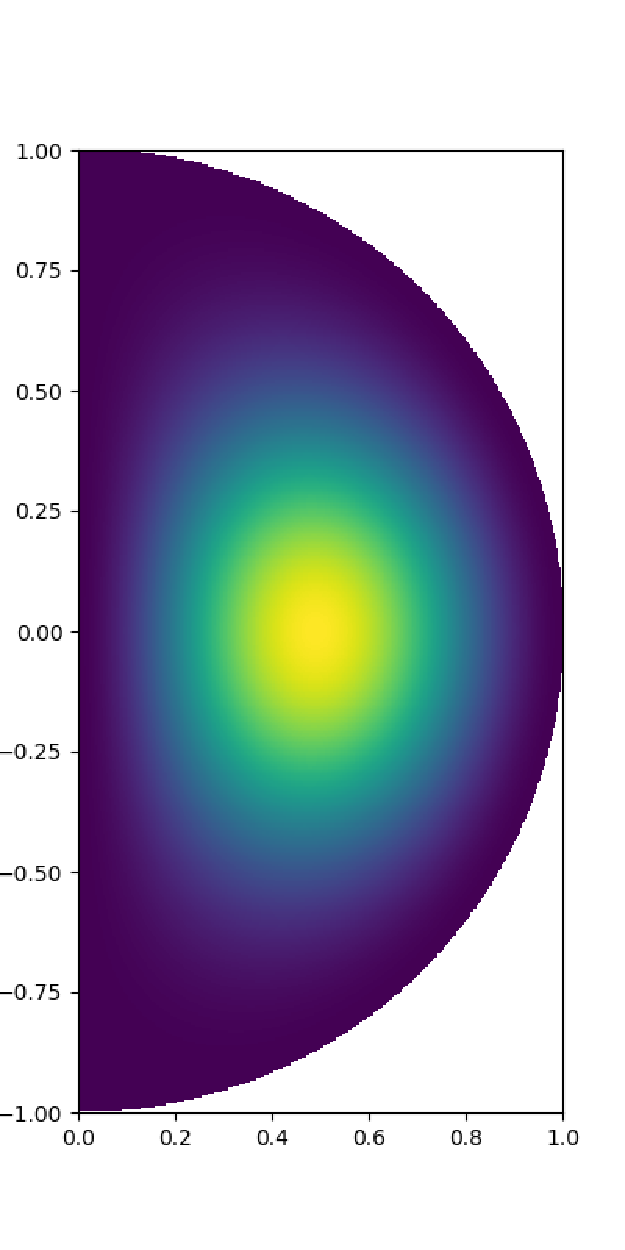
\includegraphics[scale=0.3]{solution-biharmonic}
	%\label{fig:solution-biharmonic}
	\end{subfigure}
	\begin{subfigure}{0.5\textwidth}
	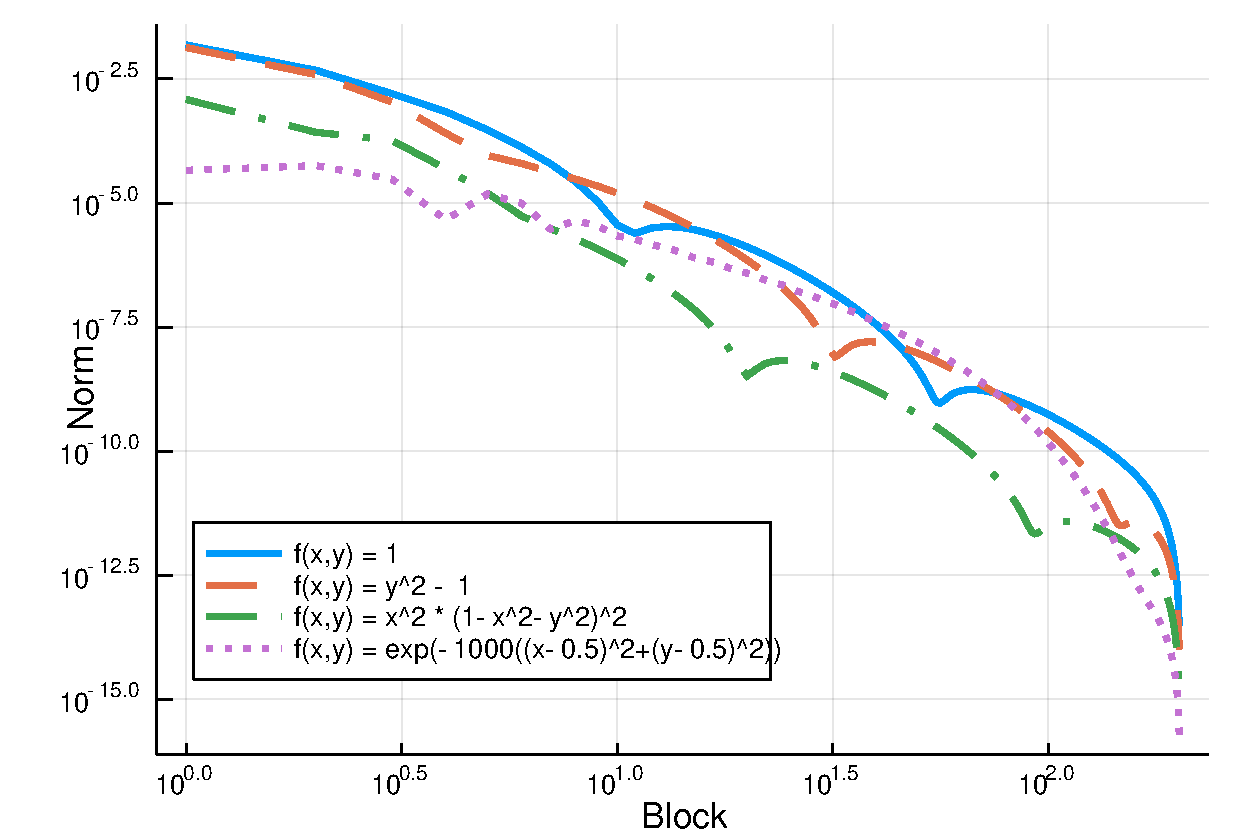
\includegraphics[scale=0.5]{solutionblocknorms-biharmonic}
	\centering
        	%\label{fig:solutionblocknorms-biharmonic}
	\end{subfigure}
	\caption{Left: The computed solution to $\Delta^2 u = f$ with zero Dirichlet and Neumann boundary conditions with $f(x,y) = 1 + \text{erf}(5(1 - 10((x - 0.5)^2 + y^2)))$. Right: The norms of each block of the computed solution of the biharmonic equation with the given right hand side functions.}
	\centering
	\label{fig:biharmonic}
\end{figure}
% END FIGURES

The Poisson equation is the classic problem of finding \(u(x,y)\) given a function \(f(x,y)\) such that:
\begin{align}
	\begin{cases}
    		\Delta u(x,y) = f(x,y) \quad \text{in } \Omega \\
		u(x,y) = 0 \quad \text{on } \partial \Omega
	\end{cases}.
	\label{eqn:poisson}
\end{align}
noting the imposition of zero Dirichlet boundary conditions on $u$.

We can tackle the problem as follows. Denote the coefficient vector for expansion of $u$ in the $\bigWii$ OP basis up to degree $N$ by $\mathbf{u}$, and the coefficient vector for expansion of $f$ in the $\bighdopii$ OP basis up to degree $N$ by $\mathbf{f}$. Since $f$ is known, we can obtain $\mathbf{f}$ using the quadrature rule above. In matrix-vector notation, our system hence becomes:
\begin{align*}
    \laplacewii \mathbf{u} = \mathbf{f}
\end{align*}
which can be solved to find $\mathbf{u}$.
In Figure \ref{fig:poisson} we see the solution to the Poisson equation with zero boundary conditions given in (\ref{eqn:poisson}) in the half-disk $\Omega$. In Figure \ref{fig:poisson} we also show the norms of each block of calculated coefficients of the approximation for four right-hand sides of the Poisson equation with N = 200, that is, 20,301 unknowns. The rate of decay in the coefficients is a proxy for the rate of convergence of the computed solution. We see that we achieve algebraic convergence for the first three examples, noting that for right hand-sides that vanish at the corners of our half-disk ($x=0, \: y = \pm 1$) we observe faster convergence. For the final Gaussian bump example, we see that we achieve spectral convergence.

\subsection{Inhomogeneous variable-coefficient Helmholtz}

Find \(u(x,y)\) given functions $v$, $f : \Omega \to \R$ such that:
\begin{align}
	\begin{cases}
    		\Delta u(x,y) + k^2 \: v(x,y) \; u(x,y) = f(x,y) \quad \text{in } \Omega \\
		u(x,y) = 0 \quad \text{on } \partial \Omega
	\end{cases}.
	\label{eqn:helmholtz}
\end{align}
where $k \in \R$, noting the imposition of zero Dirichlet boundary conditions on $u$.

We can tackle the problem as follows. Denote the coefficient vector for expansion of $u$ in the $\bigWii$ OP basis up to degree $N$ by $\mathbf{u}$, and the coefficient vector for expansion of $f$ in the $\bighdopii$ OP basis up to degree $N$ by $\mathbf{f}$. Since $f$ is known, we can obtain  the coefficients $\mathbf{f}$ using the quadrature rule above. We can obtain the matrix operator for the variable-coefficient function $v(x,y)$ by using the Clenshaw algorithm with matrix inputs as the Jacobi matrices ${J_x^{(0,0)}}^\top, {J_y^{(0,0)}}^\top$, yielding an operator matrix of the same dimension as the input Jacobi matrices a la the procedure introduced in \cite{olver2019triangle}. We can denote the resulting operator acting on coefficients in the $\bighdopoo$ space by $V({J_x^{(0,0)}}^\top, {J_y^{(0,0)}}^\top)$. In matrix-vector notation, our system hence becomes:
\begin{align*}
    (\laplacewii + k^2 T^{(0,0)\to(1,1)} \: V({J_x^{(0,0)}}^\top, {J_y^{(0,0)}}^\top) \: T_W^{(1,1)\to(0,0)}) \mathbf{u} = \mathbf{f}
\end{align*}
which can be solved to find $\mathbf{u}$. We can see the sparsity and structure of this matrix system in Figure \ref{fig:sparsity} with $v(x,y) = xy^2$ as an example. In Figure \ref{fig:helmholtz} we see the solution to the inhomogeneous variable-coefficient Helmholtz equation with zero boundary conditions given in (\ref{eqn:helmholtz}) in the half-disk $\Omega$, with $k=100$, $v(x,y) = (1 - (3(x-1)^2 + 5y^2))$ and $f(x,y) = x(1-x^2-y^2)e^x$. In Figure \ref{fig:helmholtz} we also show the norms of each block of calculated coefficients of the approximation for four right-hand sides of the inhomogeneous variable-coefficient Helmholtz equation with $k=20$ and $v(x,y) = (1 - (3(x-1)^2 + 5y^2))$ using N = 200, that is, 20,301 unknowns. The rate of decay in the coefficients is a proxy for the rate of convergence of the computed solution. We see that we achieve algebraic convergence for the first three examples, noting that for right hand sides that vanish at the corners of our half-disk ($x=0, \: y = \pm 1$) we see faster convergence. For the final Gaussian bump example, we see that we achieve spectral convergence.

We can extend this to constant non-zero boundary conditions by simply noting that the problem 
\begin{align*}
	\begin{cases}
    		\Delta u(x,y) + k^2 \: v(x,y) \; u(x,y) = f(x,y) \quad \text{in } \Omega \\
		u(x,y) = c \in \R \quad \text{on } \partial \Omega
	\end{cases}
\end{align*}
is equivalent to letting $u = \tilde{u} + c$ and solving
\begin{align*}
	\begin{cases}
    		\Delta \tilde{u}(x,y) + k^2 \: v(x,y) \; \tilde{u}(x,y) = f(x,y) - c \: k^2 \: v(x,y) \; =: g(x,y)  \quad \text{in } \Omega \\
		\tilde{u}(x,y) = 0 \quad \text{on } \partial \Omega.
	\end{cases}.
\end{align*}


\subsection{Biharmonic equation}

Find \(u(x,y)\) given a function \(f(x,y)\) such that:
\begin{align}
	\begin{cases}
    		\Delta^2 u(x,y) = f(x,y) \quad \text{in } \Omega \\
		u(x,y) = 0, \quad \frac{\partial u}{\partial n}(x,y) = 0 \quad \text{on } \partial \Omega
	\end{cases}.
	\label{eqn:biharmonic}
\end{align}
where $\Delta^2$ is the Biharmonic operator, noting the imposition of zero Dirichlet and Neumann boundary conditions on $u$. In Figure \ref{fig:biharmonic} we see the solution to the Biharmonic equation (\ref{eqn:biharmonic}) in the half-disk $\Omega$. In Figure \ref{fig:biharmonic} we also show the norms of each block of calculated coefficients of the approximation for four right-hand sides of the biharmonic equation with N = 200, that is, 20,301 unknowns.  We see that we achieve algebraic convergence for the first three examples, noting that for right hand sides that vanish at the corners of our half-disk ($x=0, \: y = \pm 1$) we see faster convergence. For the final Gaussian bump example, we see that we achieve spectral convergence.


%
\section{Conclusions}

We have shown that bivariate orthogonal polynomials can lead to sparse discretizations of general linear PDEs on specific domains whose boundary is specified by an algebraic curve---notably here the half-disk---with Dirichlet boundary conditions. This forms a building block in developing an $hp-$finite element method to solve PDEs on other polygonal domains by using suitable shaped elements, for example, by dividing the disk into disk slice elements. 
%A further extension is to develop similar relationships for 3D domains such as the half-sphere surface. With this, we can obtain a family of OPs on the half-sphere, with sparse relations, and construct sparse spectral methods for surface PDEs on half-spheres. 
This work serves as a stepping stone to constructing similar methods on other 3D spherical domains, such as spherical caps and spherical triangles.

%
\appendix
%
\section{P-finite element methods using sparse operators}\label{Appendix:PFEM}

We follow the method of \cite{beuchler2006new} to construct a sparse $p$-finite element method in terms of the operators constructed above, with the benefit of ensuring that the resulting discretisation is symmetric. Consider the 2D Dirichlet problem on a domain $\Omega$:
\begin{align*}
	\begin{cases}
         - \Delta u(x,y) = f(x,y) \quad \text{in } \Omega \\
         u = 0 \quad \text{on } \partial \Omega
         \end{cases}
\end{align*}
This has the weak formulation for any test function $v \in V := H_0^1(\Omega) = \{v \in H^1(\Omega) \quad | \quad v|_{\partial \Omega} = 0 \}$,
\begin{align*}
	L(v) := \int_\Omega f \: v \: d\mathbf{x} = \int_\Omega \nabla u \cdot \nabla v \: d\mathbf{x} =: a(u,v).
\end{align*}

In general, we would let $\FEset$ be the set of elements $\element$ that make up our finite element discretisation of the domain, where each $\element$ is a trapezium or disk slice for example. 


In this section, we limit our discretisation to a single element, that is we let $\element = \Omega$ for a half-disk/disk slice/trapezium domain. We can choose our finite dimensional space $V_p = \{v_p \in V \quad | \quad {\rm deg}\,(v_p|_\element) \le p\}$ for some $p \in \N$.

We seek $u_p \in V_p$ s.t.
\begin{align}
	L(v_p) = a(u_p,v_p) \quad \forall \: v_p \in V_p.
	\label{eqn:FEMweakform}
\end{align}

Define $\Lambda^{(a,b)} := \langle \bighdop^{(a,b)}, \: {\bighdop^{(a,b)}}^\top \rangle_{W^{(a,b)}}$ where $W^{(a,b)}$ is the weight with which the OPs in $\bighdop^{(a,b)}$ are orthogonal with respect to. Note that due to orthogonality this is a diagonal matrix. We can choose a basis for $V_p$ by using the weighted orthogonal polynomials on $\element$ with parameters $a = b = 1$:
\begin{align*}
\bigWii(x,y) &:= \begin{pmatrix}
		\bigWii_0(x,y) \\
		\bigWii_1(x,y) \\
		\bigWii_2(x,y) \\
		\vdots \\
		\bigWii_p(x,y)
	\end{pmatrix}, \\
\bigWii_n(x,y) &:= \begin{pmatrix}
		\Wii(x,y) \: \hdopii_{n,0}(x,y) \\
		\vdots \\
		\Wii(a,y) \: \hdopii_{n,n}(x,y)
	\end{pmatrix} \in \R^{n+1} \quad \forall n = 0,1,2,\dots,p,
\end{align*}
and rewrite (\ref{eqn:FEMweakform}) in matrix form:
\begin{align*}
	a(u_p,v_p) &= \int_\element \nabla u_p \cdot \nabla v_p \: d\mathbf{x} \\
	&= \int_\element \begin{pmatrix}
					\partial_x v_p \\
					\partial_y v_p
				\end{pmatrix}^\top 
				\begin{pmatrix}
					\partial_x u_p \\
					\partial_y u_p
				\end{pmatrix}
				\\
	&= \int_\element \begin{pmatrix}
					\bighdopoo^\top \Wii_x \mathbf{v} \\
					\bighdopoo^\top T_W^{(1,0)\to(0,0)} \Wii_y \mathbf{v}
				\end{pmatrix}^\top 
				\begin{pmatrix}
					\bighdopoo^\top \Wii_x \mathbf{u} \\
					\bighdopoo^\top T_W^{(1,0)\to(0,0)} \Wii_y \mathbf{u}
				\end{pmatrix}
				\\
	&= \int_\element \Big( \mathbf{v}^\top {\Wii_x}^\top \bighdopoo \bighdopoo^\top \Wii_x \mathbf{u} \nonumber \\
					& \quad \quad \quad + \mathbf{v}^\top ({T_W^{(1,0)\to(0,0)} \Wii_y})^\top \bighdopoo \bighdopoo^\top T_W^{(1,0)\to(0,0)} \Wii_y \mathbf{u}  \Big) \: d\mathbf{x} \\
	&= \mathbf{v}^\top \: \Big( {\Wii_x}^\top \Lambda^{(0,0)} \Wii_x + ({T_W^{(1,0)\to(0,0)} \Wii_y})^\top \Lambda^{(0,0)} T_W^{(1,0)\to(0,0)} \Wii_y \Big) \: \mathbf{u}
\end{align*}
where $\mathbf{u}, \mathbf{v}$ are the coefficient vectors of the expansions of $u_p, v_p \in V_p$ respectively in the $V_p$ basis ($\bigWii$ OPs), and
\begin{align*}
	L(v_p) &= \int_\element \: v_p \: f \: d\mathbf{x} \\
	&= \int_\element \: \mathbf{v}^\top \: \bigWii \: \bighdopii^\top \: \mathbf{f} \: d\mathbf{x} \\
	&= \mathbf{v}^\top \: \langle \bighdopii, {\bighdopii}^\top \rangle_{\Wii} \: d\mathbf{x} \\
	&= \mathbf{v}^\top \Lambda^{(1,1)} \: \mathbf{f},
\end{align*}
where $\mathbf{f}$ is the coefficient vector for the expansion of the function $f(x,y)$ in the $\bighdopii$ OP basis.

Since (\ref{eqn:FEMweakform}) is equivalent to stating that
\begin{align*}
	L(\Wii \hdopii_{n,k}) = a(u_p,\Wii \hdopii_{n,k}) \quad \forall \: n = 0,\dots,p, \: k = 0,\dots,n,
\end{align*}
(i.e. holds for all basis functions of $V_p$) by choosing $v_p$ as each basis function, we can equivalently write the linear system for our finite element problem as:
\begin{align*}
A\mathbf{u} = \tilde{\mathbf{f}}.
\end{align*}
where the (element) stiffness matrix $A$ is defined by 
\begin{align*}
A = {\Wii_x}^\top \Lambda^{(0,0)} \Wii_x + ({T_W^{(1,0)\to(0,0)} \Wii_y})^\top \Lambda^{(0,0)} T_W^{(1,0)\to(0,0)} \Wii_y, 
\end{align*}
and the load vector $\tilde{\mathbf{f}}$ is given by 
\begin{align*}
\tilde{\mathbf{f}} = \Lambda^{(1,1)} \: \mathbf{f}.
\end{align*}

Note the since we have sparse operator matrices for partial derivatives and basis-transform, we obtain a symmetric sparse (element) stiffness matrix, as well as a sparse operator matrix for calculating the load vector (rhs).

\section{Disk slices}\label{Appendix:DiskSlices}

The work in this paper on the half-disk can be easily transferred to the domain of a disk slice by which we mean
\begin{align*}
	\Omega := \{(x,y) \in \R^2 \quad | \quad \alpha < x < \beta, \: \gamma \rho(x) < y < \delta \rho(x)\}
\end{align*}
with
\begin{align*}
\begin{cases}
(\alpha, \beta) &\subset (-1,1) \\
(\gamma, \delta) &:= (-1,1) \\
\rho(x) &:= (1-x^2)^{\half}.
\end{cases}
\end{align*}
Our 1D weight functions on the intervals $(\alpha, \beta)$ and $(\gamma, \delta)$ respectively are then given by:
\begin{align*}
\begin{cases}
\genjacw^{(a,b,c)}(x) &:= (\beta - x)^a \: (x - \alpha)^{b} \: \rho(x)^{c} \\
\jacw^{(a)}(x) &:= (1-x^2)^a.
\end{cases}
\end{align*}

The weight $\jacw^{(a)}(x)$ is a still an ultraspherical weight, and the corresponding OPs are the Jacobi polynomials $\{\jac_n^{(a, a)}\}$. $\genjacw^{(a,b,c)}(x)$ is the (non-classical) weight for the OPs denoted $\{\genjac_n^{(a,b,c)}\}\). Thus we arrive at the three-parameter family of 2D orthogonal polynomials $\{\hdopnk^{(a,b,c)}\}$ on $\Omega$ given by, for \(0 \le k \le n, \: n = 0,1,2,\dots,\)
\begin{align*}
	\hdopnk^{(a,b,c)}(x,y) := \genjacnmk^{(a, b, 2c+2k+1)}(x) \: \rho(x)^k \: \jac_k^{(c,c)}\fpr(\frac{y}{\rho(x)}), \quad (x,y) \in \Omega, 
\end{align*}
orthogonal with respect to the weight
\begin{align*}
	W^{(a,b,c)}(x,y) &:= \genjacw^{(a,b,2c)}(x) w^{(c)}_P\fpr(\frac{y}{\rho(x)}) \nonumber \\
	&= (\beta - x)^a \: (x - \alpha)^{b} \: (\rho(x)^2 -y^2)^c \nonumber \\
	&= (\beta - x)^a \: (x - \alpha)^{b} \: (1 - x^2 -y^2)^c , \quad (x,y) \in \Omega.
\end{align*}

We note again that by making the adjustment that $\genjacw^{(a,b,c)}(x) = (\beta - x)^a \: (x - \alpha)^{b} \: \rho(x)^{2c}$, and setting the first parameter $a$ to zero and removing it for the family and weight for $\{\genjac_n^{(a,b,c)}\}$, and taking and $\alpha = 0$, $\beta = 1$, we recover the half-disk case.

The sparsity of operator matrices for partial differentiation by $x, y$ as well as for parameter transformations generalise to such disk slice domains. For instance, if we inspect the proof of Lemma \ref{theorem:sparsityofdifferentialoperators}, we see that it can easily generalise to the weights and domain $\Omega$ for a disk slice.


\section{Trapeziums}\label{Appendix:Trapezium}

We can further extend this work to trapezium shaped domains. Note that for any trapezium there exists an affine map to the canonical trapezium domain that we consider here, given by
\begin{align*}
	\Omega := \{(x,y) \in \R^2 \quad | \quad \alpha < x < \beta, \: \gamma \rho(x) < y < \delta \rho(x)\}
\end{align*}
with 
\begin{align*}
\begin{cases}
(\alpha, \beta) &:= (0,1) \\
(\gamma, \delta) &:= (0,1) \\
\rho(x) &:= 1-\half x \\
\genjacw^{(a,b,c)}(x) &:= (\beta - x)^a \: (x - \alpha)^{b} \: \rho(x)^{c} = (1-x)^{a} \: x^b \: (1-\half x)^{c} \\
\jacw^{(a,b)}(x) &:= (\delta-x)^a \: (x - \gamma)^b = (1-x)^a \: x^b.
\end{cases}
\end{align*}
The weight $\jacw^{(a,b)}(x)$ is the weight for the shifted Jacobi polynomials on the interval $[0,1]$, and hence the corresponding OPs are the shifted Jacobi polynomials $\{\tilde{P}_n^{(a, b)}\}$. We note that the shifted Jacobi polynomials relate to the normal Jacobi polynomials by the relationship $\tilde{P}_n^{(a,b)}(x) = \jac_n^{(a,b)}(2x-1)$ for any degree $n = 0,1,2,\dots$ and $x \in [0,1]$. $\genjacw^{(a,b,c)}(x)$ is the (non-classical) weight for the OPs we dentote $\{\genjac_n^{(a,b,c)}\}\). Thus we arrive at the four-parameter family of 2D orthogonal polynomials $\{\hdopnk^{(a,b,c,d)}\}$ on $\Omega$ given by, for \(0 \le k \le n, \: n = 0,1,2,\dots,\)
\begin{align*}
	\hdopnk^{(a,b,c,d)}(x,y) := \genjacnmk^{(a, b, c+d+2k+1)}(x) \: \rho(x)^k \: \tilde{P}_k^{(d,c)}(\frac{y}{\rho(x)}), \quad (x,y) \in \Omega, 
\end{align*}
orthogonal with respect to the weight
\begin{align*}
	W^{(a,b,c,d)}(x,y) &:= \genjacw^{(a,b,c+d)}(x) \: w^{(d,c)}_P(\frac{y}{\rho(x)}) \nonumber \\
	&= (1-x)^a \: x^b \: y^c \: (1-\half x - y)^d, \quad (x,y) \in \Omega.
\end{align*}


\bibliography{halfdisk}


\end{document}











  